\documentclass[12pt,a4paper]{article}

\usepackage[utf8]{inputenc}
\usepackage[T1]{fontenc}
\usepackage[spanish,es-tabla]{babel}
\usepackage{geometry}
\usepackage{graphicx}
\usepackage{float}
\usepackage{array}
\usepackage{booktabs}
\usepackage{longtable}
\usepackage{caption}
\usepackage{subcaption}
\usepackage{hyperref}
\usepackage{enumitem}
\usepackage{pdflscape}
\usepackage{xcolor}

\geometry{margin=2.5cm}
\setlength{\parskip}{0.7em}
\setlength{\parindent}{0pt}
\captionsetup{font=small,labelfont=bf}
\hypersetup{
    colorlinks=true,
    linkcolor=blue!50!black,
    urlcolor=blue!60!black,
    pdftitle={Documentación Práctica 2 - Organización Computacional},
    pdfauthor={Alex Ricardo Castañeda Rodríguez}
}

\title{Documentación Técnica\\Práctica 2 - Organización Computacional}
\author{Grupo de trabajo}
\date{22 de marzo de 2026}

\begin{document}

\begin{titlepage}
    \centering
    \vspace*{1.5cm}
    
\includegraphics[width=0.23\textwidth]{assets/usac_logo.png}\par\vspace{1cm}
    {\scshape\LARGE Universidad de San Carlos de Guatemala \par}
    \vspace{0.4cm}
    {\scshape\Large Facultad de Ingeniería \par}
    \vspace{0.2cm}
    {\scshape\large Escuela de Ciencias y Sistemas \par}
    \vspace{1.8cm}
    {\Huge\bfseries Práctica 2\\[0.2cm] Organización Computacional\par}
    \vspace{0.8cm}
    {\Large Documentación del prototipo \textit{LogicCalc}\par}
    \vspace{1cm}
    \begin{tabular}{|c|p{8.2cm}|}
        \hline
        \textbf{Carnet} & \textbf{Integrante} \\
        \hline
        202406918 & Claudia Maribel Tigüilá Tecum \\
        \hline
        202403929 & Emiliana Elizabeth Pú Lara \\
        \hline
        202300476 & Alex Ricardo Castañeda Rodríguez \\
        \hline
        201904522 & Byron Manuel Hernández López \\
        \hline
    \end{tabular}
    \vfill
    {\large Marzo de 2026\par}
    \vfill
\end{titlepage}

\tableofcontents
\newpage

\section{Resumen}
En esta práctica se desarrolló un prototipo de calculadora digital llamado \textit{LogicCalc}, construido a partir de compuertas lógicas TTL, multiplexores, comparadores, sumadores de 4 bits, decodificadores y displays de siete segmentos. El sistema opera sobre dos operandos binarios de 4 bits, denominados $A$ y $B$, y ejecuta operaciones aritméticas, lógicas y comparativas de acuerdo con la selección del usuario.

La implementación se realizó en Proteus como base de diseño y posteriormente se trasladó a protoboards para la validación física. La documentación integra el marco formativo solicitado, la descripción de la solución implementada, capturas del circuito, presupuesto derivado de la factura proporcionada y anexos fotográficos del montaje.

\section{Marco Formativo}

\subsection{Valor}
La práctica fortalece la comprensión del diseño digital combinacional mediante la construcción de una ALU básica por bloques. El valor principal de la actividad radica en conectar teoría y práctica: no solo se plantea la lógica booleana de cada operación, sino que también se valida la factibilidad del circuito al implementarlo con componentes físicos reales.

\subsection{Competencias}
Durante el desarrollo de la práctica se fortalecieron las siguientes competencias:
\begin{itemize}[leftmargin=1.2cm]
    \item Análisis y síntesis de circuitos digitales combinacionales.
    \item Interpretación de hojas de datos y uso correcto de familias TTL serie 74LS.
    \item Diseño modular de sistemas digitales complejos a partir de subbloques.
    \item Validación funcional por simulación en Proteus y por montaje físico en protoboard.
    \item Documentación técnica de arquitectura, materiales, resultados y costos.
\end{itemize}

\subsection{Objetivo SMART}
Diseñar, simular e implementar antes del 22 de marzo de 2026 un prototipo funcional de calculadora digital de 4 bits, capaz de ejecutar operaciones aritméticas, lógicas y comparativas sobre dos entradas binarias, mostrando los resultados mediante LEDs y displays de siete segmentos, con evidencia visual, presupuesto y documentación técnica completa.

\section{Enunciado de la Práctica}

\subsection{Descripción del problema a resolver}
De acuerdo con el enunciado, la práctica consistió en diseñar e implementar un prototipo denominado \textit{LogicCalc}, basado en una Unidad Aritmético Lógica básica. El sistema debía trabajar bajo lógica combinacional, operar con dos números binarios de 4 bits y presentar distintas salidas según la operación activa.

La solución debía integrar al menos tres grandes bloques funcionales:
\begin{itemize}[leftmargin=1.2cm]
    \item Unidad aritmética.
    \item Unidad lógica.
    \item Unidad comparativa.
\end{itemize}

\subsection{Alcance de la práctica}
El alcance cubrió el diseño lógico, la simulación, la selección de componentes, el montaje físico, la comprobación visual de resultados y la elaboración de documentación. No se consideró el uso de microcontroladores ni lógica secuencial; el sistema fue resuelto únicamente con componentes digitales discretos de la serie 74LS y elementos pasivos de apoyo.

\section{Requisitos Funcionales}
Con base en el PDF de la práctica, los requisitos funcionales principales atendidos por el prototipo fueron los siguientes:

\subsection{Unidad Aritmética}
\begin{itemize}[leftmargin=1.2cm]
    \item Suma binaria entre $A$ y $B$.
    \item Resta binaria entre $A$ y $B$, con validación de signo para identificar cuando $A < B$.
    \item Multiplicación binaria entre $A$ y $B$.
    \item Potencia de $A$, elevando al cuadrado cuando $B = 2$ y al cubo cuando $B = 3$.
    \item Visualización de resultados en salidas binarias y en displays de siete segmentos.
\end{itemize}

\subsection{Unidad Lógica}
\begin{itemize}[leftmargin=1.2cm]
    \item Operación AND bit a bit entre $A$ y $B$.
    \item Operación OR bit a bit entre $A$ y $B$.
    \item Operación NAND bit a bit entre $A$ y $B$.
    \item Operación XNOR bit a bit entre $A$ y $B$.
    \item Presentación del resultado mediante 4 LEDs.
\end{itemize}

\subsection{Unidad Comparativa}
\begin{itemize}[leftmargin=1.2cm]
    \item Mostrar el dígito mayor y el dígito menor entre $A$ y $B$.
    \item Si $A = B$, desplegar el mismo valor en ambos displays.
    \item Utilizar indicadores de unidad activa para diferenciar la unidad aritmética de la lógica.
\end{itemize}

\section{Arquitectura de la Solución}

\subsection{Descripción general}
La arquitectura se organizó en bloques independientes conectados a un controlador principal. Dicho controlador recibe un selector de 3 bits y habilita una sola operación a la vez. La salida activa se propaga a los submódulos correspondientes, evitando conflictos entre unidades.

Los operandos $A$ y $B$ se ingresan mediante DIP switches de 4 posiciones. Las operaciones aritméticas producen resultados intermedios en binario, los cuales luego se convierten a BCD cuando es necesario para visualizarlos en displays de siete segmentos. Las operaciones lógicas se muestran por medio de LEDs dedicados.

\begin{table}[H]
    \centering
    \caption{Tabla de selección general de operaciones.}
    \begin{tabular}{c c c p{8cm}}
        \toprule
        \textbf{A} & \textbf{B} & \textbf{C} & \textbf{Operación habilitada} \\
        \midrule
        0 & 0 & 0 & Suma \\
        1 & 0 & 0 & Resta \\
        0 & 1 & 0 & Multiplicación \\
        1 & 1 & 0 & Potencia \\
        0 & 0 & 1 & AND \\
        1 & 0 & 1 & OR \\
        0 & 1 & 1 & NAND \\
        1 & 1 & 1 & XNOR / ruta lógica final \\
        \bottomrule
    \end{tabular}
\end{table}

\begin{table}[H]
    \centering
    \caption{Resumen general de módulos implementados.}
    \small
    \begin{tabular}{p{2.8cm}p{3.1cm}p{3cm}p{3cm}p{2.9cm}}
        \toprule
        \textbf{Módulo} & \textbf{Integrados principales} & \textbf{Entradas} & \textbf{Salidas} & \textbf{Función} \\
        \midrule
        Controlador principal & 74LS138, 74LS04 & Selector de 3 bits & Líneas \texttt{op\_*}, LEDs de estado & Habilita una operación a la vez \\
        Entradas binarias & DIPSW\_4, resistencias & Interruptores para $A$ y $B$ & Buses $A[3:0]$ y $B[3:0]$ & Define los operandos de trabajo \\
        Suma y resta & 74LS86, 74LS08, 74LS32 & $A[3:0]$, $B[3:0]$, \texttt{op\_res} & \texttt{RES[3:0]}, \texttt{RES\_COUT}, \texttt{sign\_bit} & Calcula $A+B$ y $A-B$ \\
        Multiplicación & 74LS08, 74LS283 & $A[3:0]$, $B[3:0]$ & \texttt{P[7:0]} & Calcula el producto binario \\
        Potencia & 74LS08, 74LS283, 74LS157 & $A[3:0]$, $B[3:0]$, \texttt{op\_pow} & \texttt{POW[5:0]} & Calcula $A^2$ o $A^3$ \\
        Unidad lógica & 74LS08, 74LS32, 74LS00, 74LS266 & $A[3:0]$, $B[3:0]$ & LEDs lógicos & Calcula AND, OR, NAND y XNOR \\
        Unidad comparativa & 74LS85, 74LS157, 74LS48 & $A[3:0]$, $B[3:0]$ & Displays mayor y menor & Muestra el valor mayor y menor \\
        Binario a BCD & 74LS86, 74LS08, 74LS32, 74LS283 & Resultados aritméticos & BCD para displays & Convierte resultados binarios a salida visual \\
        \bottomrule
    \end{tabular}
\end{table}

\subsection{Controlador principal}
El controlador central fue construido a partir de un decodificador 74LS138 y compuertas inversoras 74LS04. Este bloque genera las líneas de habilitación para suma, resta, multiplicación, potencia y operaciones lógicas, además de los indicadores visuales de modo.

\begin{table}[H]
    \centering
    \caption{Ficha del módulo controlador principal.}
    \begin{tabular}{p{3.6cm}p{10cm}}
        \toprule
        \textbf{Elemento} & \textbf{Descripción} \\
        \midrule
        Integrados usados & 74LS138 y 74LS04 \\
        Entradas & Tres líneas del selector general y línea de control para indicadores \\
        Salidas & \texttt{op\_sum}, \texttt{op\_res}, \texttt{op\_mul}, \texttt{op\_pow}, \texttt{op\_and}, \texttt{op\_or}, \texttt{op\_nand}, \texttt{op\_xnor} \\
        Función & Decodifica la selección del usuario y activa el módulo correspondiente \\
        \bottomrule
    \end{tabular}
\end{table}

\begin{figure}[H]
    \centering
    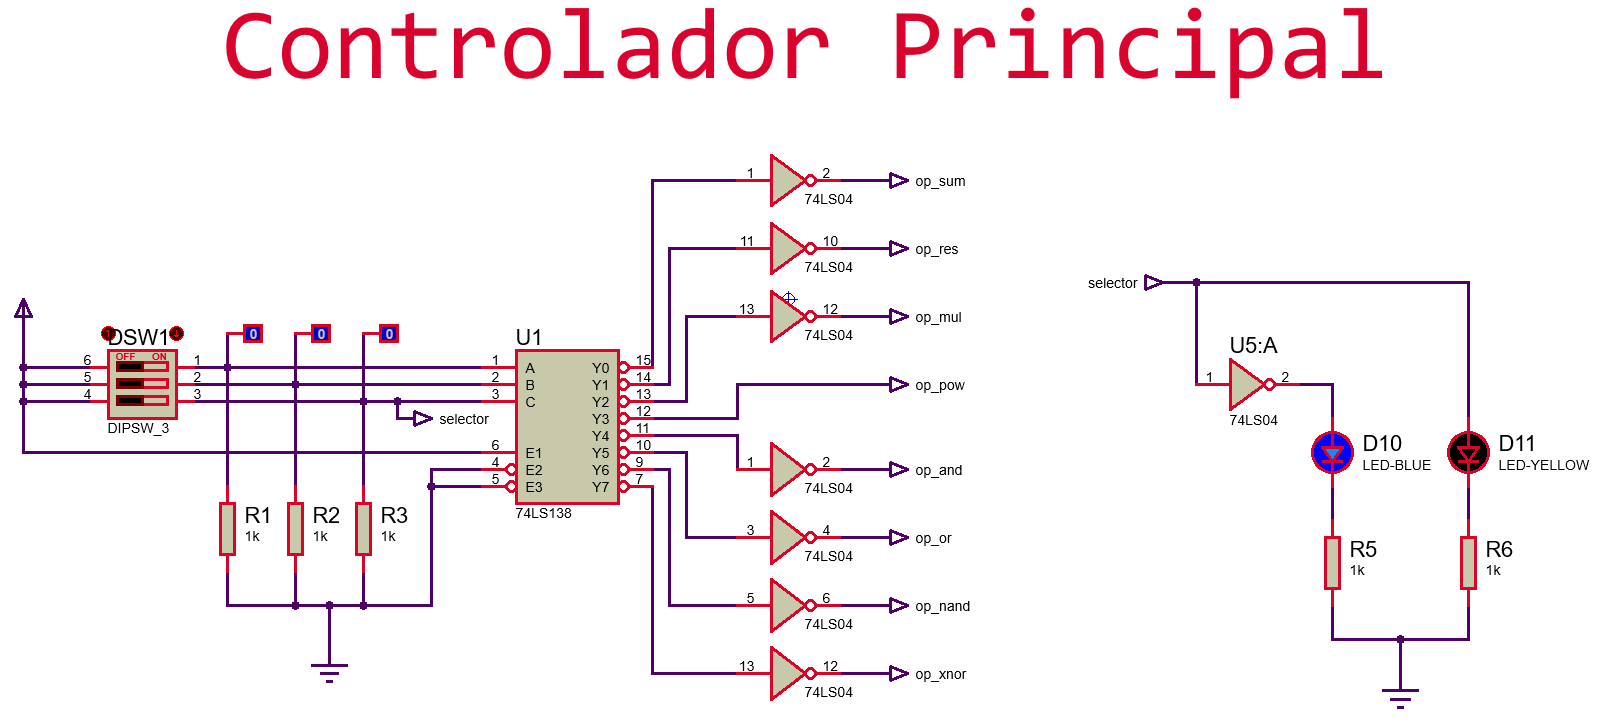
\includegraphics[width=\textwidth]{assets/controlador_principal.png}
    \caption{Controlador principal del sistema.}
\end{figure}

\subsection{Entradas binarias}
Los números de entrada se definieron con dos bancos de DIP switches de 4 bits. Cada línea utiliza resistencias de \textit{pull-down} para estabilizar las entradas y garantizar niveles lógicos correctos.

\begin{table}[H]
    \centering
    \caption{Ficha del módulo de entradas binarias.}
    \begin{tabular}{p{3.6cm}p{10cm}}
        \toprule
        \textbf{Elemento} & \textbf{Descripción} \\
        \midrule
        Componentes usados & Dos DIP switches de 4 posiciones y resistencias de 1k$\Omega$ \\
        Entradas & Acción manual del usuario sobre los interruptores \\
        Salidas & Buses $A_3,A_2,A_1,A_0$ y $B_3,B_2,B_1,B_0$ \\
        Función & Proporciona los operandos binarios de 4 bits para todas las operaciones \\
        \bottomrule
    \end{tabular}
\end{table}

\begin{table}[H]
    \centering
    \caption{Combinaciones binarias posibles para cada operando de 4 bits.}
    \begin{tabular}{c c}
        \toprule
        \textbf{Binario} & \textbf{Valor decimal} \\
        \midrule
        0000 & 0 \\
        0001 & 1 \\
        0010 & 2 \\
        0011 & 3 \\
        0100 & 4 \\
        0101 & 5 \\
        0110 & 6 \\
        0111 & 7 \\
        1000 & 8 \\
        1001 & 9 \\
        1010 & 10 \\
        1011 & 11 \\
        1100 & 12 \\
        1101 & 13 \\
        1110 & 14 \\
        1111 & 15 \\
        \bottomrule
    \end{tabular}
\end{table}

\begin{table}[H]
    \centering
    \caption{Ejemplos de combinaciones de prueba entre los operandos $A$ y $B$.}
    \small
    \begin{tabular}{>{\centering\arraybackslash}p{1.6cm} >{\centering\arraybackslash}p{1.3cm} >{\centering\arraybackslash}p{1.6cm} >{\centering\arraybackslash}p{1.3cm} >{\centering\arraybackslash}p{1.7cm} p{5.2cm}}
        \toprule
        \textbf{$A$ bin} & \textbf{$A$ dec} & \textbf{$B$ bin} & \textbf{$B$ dec} & \textbf{Relacion} & \textbf{Uso de prueba} \\
        \midrule
        0011 & 3 & 0010 & 2 & $A > B$ & Validación de comparación y resta positiva \\
        0010 & 2 & 0011 & 3 & $A < B$ & Validación de comparación y bandera de signo \\
        0101 & 5 & 0101 & 5 & $A = B$ & Validacion de displays iguales en la unidad comparativa \\
        0011 & 3 & 0001 & 1 & $A > B$ & Validación de operaciones lógicas y aritméticas simples \\
        0011 & 3 & 0010 & 2 & $A > B$ & Caso representativo de potencia con $B = 2$ \\
        0010 & 2 & 0011 & 3 & $A < B$ & Caso representativo de potencia con $B = 3$ \\
        \bottomrule
    \end{tabular}
\end{table}

\begin{figure}[H]
    \centering
    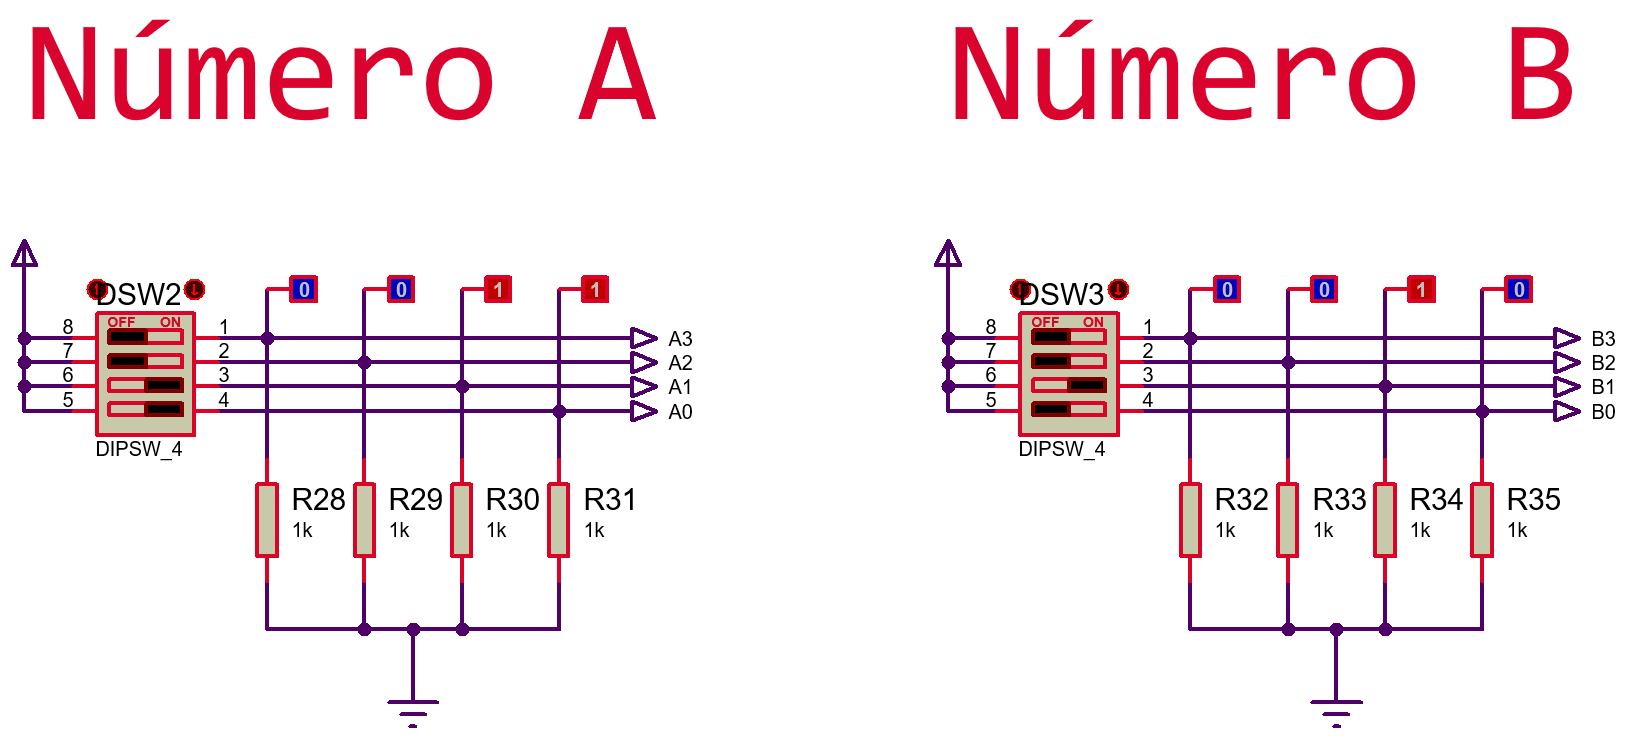
\includegraphics[width=\textwidth]{assets/numeros_A_B.png}
    \caption{Configuración de los operandos binarios $A$ y $B$.}
\end{figure}

\section{Diseño por Módulos}

\subsection{Módulo de suma y resta}
La suma y la resta se resolvieron con una estructura de sumadores completos implementados mediante compuertas XOR, AND y OR. Para la resta se empleó la técnica de complemento a dos parcial, controlada por la línea \texttt{op\_res}, la cual invierte los bits de $B$ y modifica la propagación del acarreo.

La salida incluye cuatro bits de resultado, bit de acarreo y una bandera derivada del signo. Estos datos alimentan tanto la etapa de visualización binaria como el bloque de conversión a BCD.

\begin{table}[H]
    \centering
    \caption{Comportamiento funcional del bloque suma/resta.}
    \begin{tabular}{c p{10.5cm}}
        \toprule
        \textbf{op\_res} & \textbf{Función del módulo} \\
        \midrule
        0 & El bloque trabaja como sumador binario de 4 bits, calculando $A + B$. \\
        1 & El bloque modifica los bits de $B$ con XOR y utiliza el acarreo de entrada para implementar la resta binaria $A - B$. \\
        \bottomrule
    \end{tabular}
\end{table}

\begin{table}[H]
    \centering
    \caption{Tabla de verdad del sumador completo implementado por bit.}
    \begin{tabular}{c c c c c}
        \toprule
        \textbf{A} & \textbf{B} & \textbf{$C_{in}$} & \textbf{S} & \textbf{$C_{out}$} \\
        \midrule
        0 & 0 & 0 & 0 & 0 \\
        0 & 0 & 1 & 1 & 0 \\
        0 & 1 & 0 & 1 & 0 \\
        0 & 1 & 1 & 0 & 1 \\
        1 & 0 & 0 & 1 & 0 \\
        1 & 0 & 1 & 0 & 1 \\
        1 & 1 & 0 & 0 & 1 \\
        1 & 1 & 1 & 1 & 1 \\
        \bottomrule
    \end{tabular}
\end{table}

\begin{table}[H]
    \centering
    \caption{Ejemplos de funcionamiento de la suma binaria de 4 bits.}
    \small
    \begin{tabular}{>{\centering\arraybackslash}p{2.2cm} >{\centering\arraybackslash}p{2.2cm} >{\centering\arraybackslash}p{2.6cm} p{5.5cm}}
        \toprule
        \textbf{$A$} & \textbf{$B$} & \textbf{Resultado} & \textbf{Interpretacion} \\
        \midrule
        0011 & 0010 & 0101 & $3 + 2 = 5$ \\
        0101 & 0011 & 1000 & $5 + 3 = 8$ \\
        1111 & 0001 & 1 0000 & $15 + 1 = 16$, se activa el acarreo de salida \\
        0111 & 0110 & 1101 & $7 + 6 = 13$ \\
        \bottomrule
    \end{tabular}
\end{table}

\begin{table}[H]
    \centering
    \caption{Ejemplos de funcionamiento de la resta binaria de 4 bits.}
    \small
    \begin{tabular}{>{\centering\arraybackslash}p{2.2cm} >{\centering\arraybackslash}p{2.2cm} >{\centering\arraybackslash}p{2.8cm} p{5.3cm}}
        \toprule
        \textbf{$A$} & \textbf{$B$} & \textbf{Resultado} & \textbf{Interpretacion} \\
        \midrule
        0011 & 0010 & 0001 & $3 - 2 = 1$ \\
        0101 & 0011 & 0010 & $5 - 3 = 2$ \\
        0010 & 0011 & 1111 & $2 - 3 = -1$ en complemento a dos; se usa la bandera de signo \\
        1000 & 0001 & 0111 & $8 - 1 = 7$ \\
        \bottomrule
    \end{tabular}
\end{table}

\begin{table}[H]
    \centering
    \caption{Ficha del módulo de suma y resta.}
    \begin{tabular}{p{3.6cm}p{10cm}}
        \toprule
        \textbf{Elemento} & \textbf{Descripción} \\
        \midrule
        Integrados usados & 74LS86, 74LS08, 74LS32 y 74LS04 para manejo de signo \\
        Entradas & $A[3:0]$, $B[3:0]$, \texttt{op\_res} y acarreos intermedios \\
        Salidas & \texttt{RES[3:0]}, \texttt{RES\_COUT}, \texttt{sign}, \texttt{sign\_bit} \\
        Función & Ejecuta suma o resta binaria de 4 bits según la operación activa \\
        \bottomrule
    \end{tabular}
\end{table}

\begin{figure}[H]
    \centering
    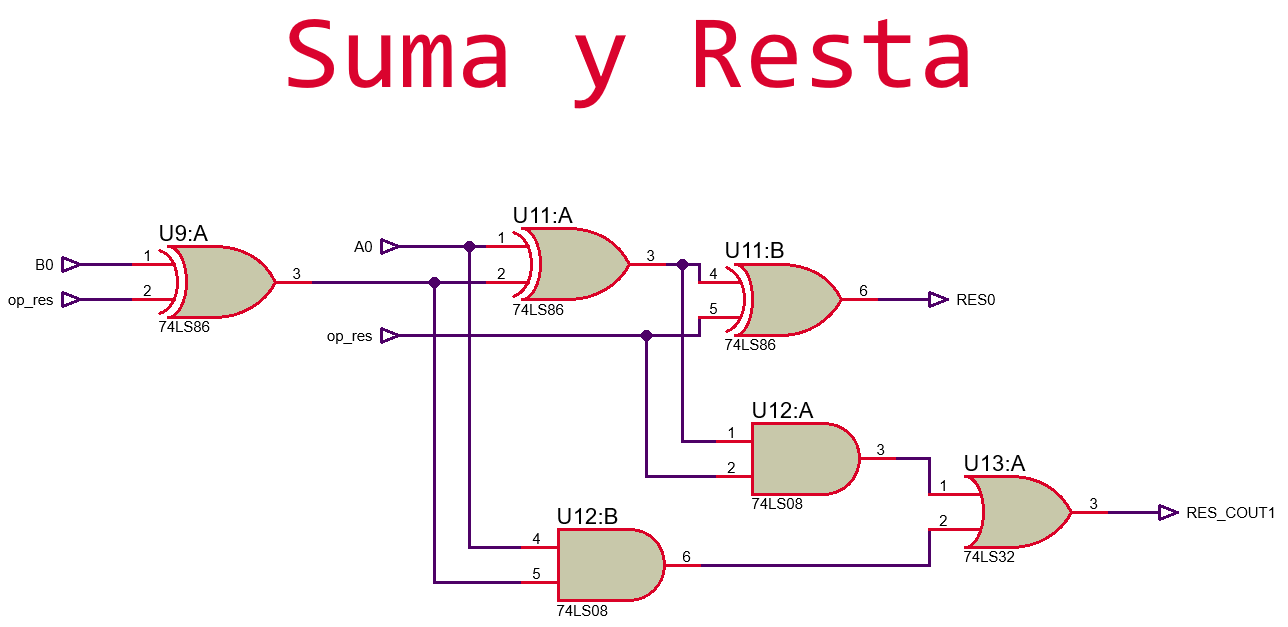
\includegraphics[width=\textwidth]{assets/suma_resta_p1.png}
    \caption{Etapa 0 del módulo de suma y resta.}
\end{figure}

\begin{figure}[H]
    \centering
    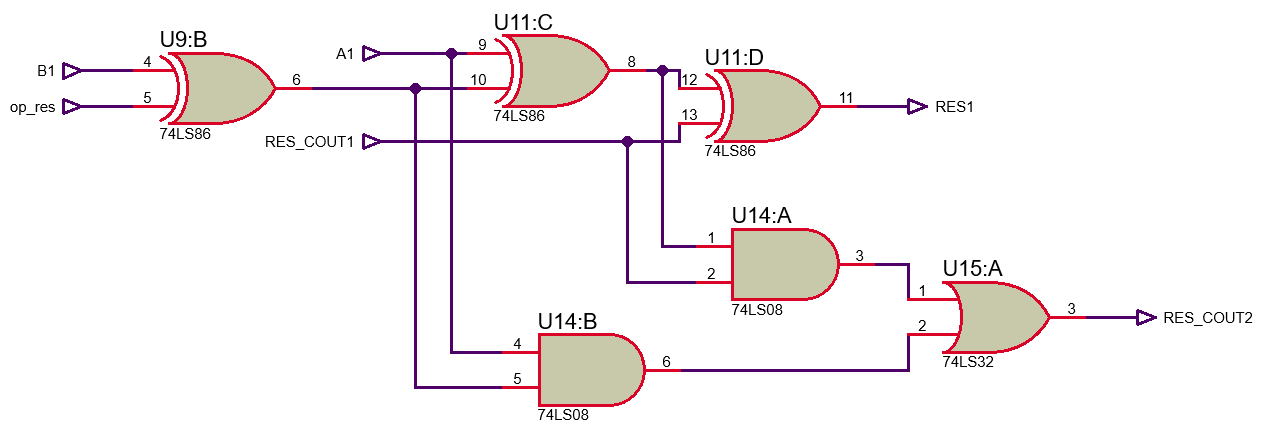
\includegraphics[width=\textwidth]{assets/suma_resta_p2.png}
    \caption{Etapa 1 del módulo de suma y resta.}
\end{figure}

\begin{figure}[H]
    \centering
    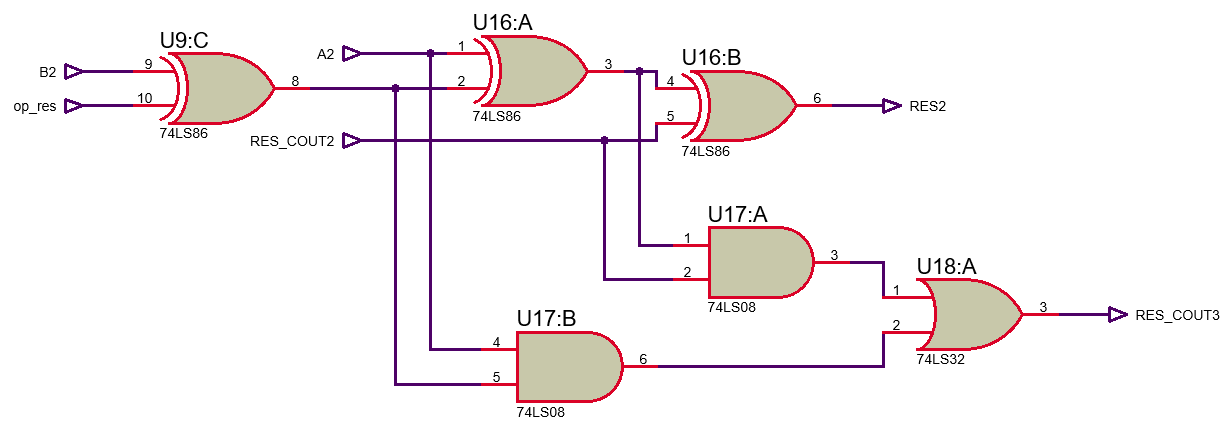
\includegraphics[width=\textwidth]{assets/suma_resta_p3.png}
    \caption{Etapa 2 del módulo de suma y resta.}
\end{figure}

\begin{figure}[H]
    \centering
    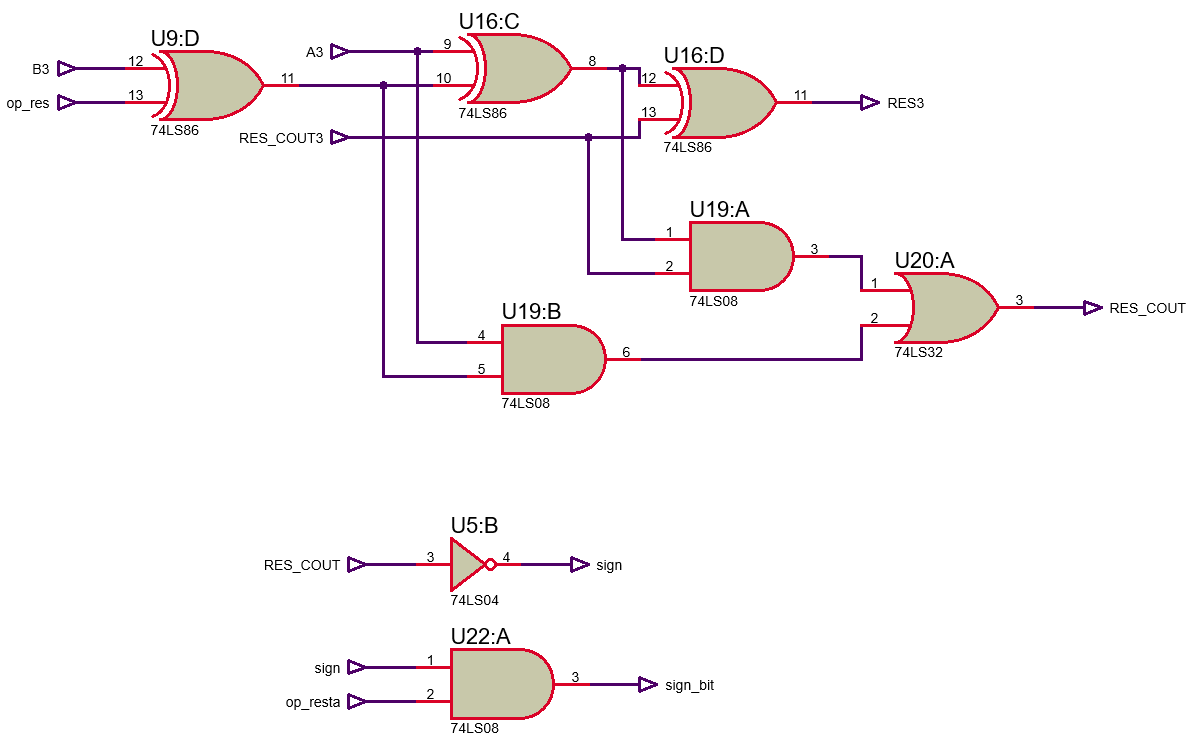
\includegraphics[width=0.92\textwidth]{assets/suma_resta_p4.png}
    \caption{Etapa 3 y generación de señal de signo para la resta.}
\end{figure}

\subsection{Módulo de multiplicación}
La multiplicación binaria se implementó mediante productos parciales con compuertas AND y su acumulación progresiva usando sumadores 74LS283. Este enfoque replica la multiplicación binaria clásica por desplazamientos y sumas.

\begin{table}[H]
    \centering
    \caption{Generación conceptual de productos parciales en la multiplicación binaria.}
    \small
    \begin{tabular}{p{3cm}p{9.5cm}}
        \toprule
        \textbf{Producto parcial} & \textbf{Descripción} \\
        \midrule
        $A \cdot B_0$ & Se obtiene aplicando AND entre cada bit de $A$ y el bit menos significativo de $B$. \\
        $A \cdot B_1$ & Se obtiene aplicando AND entre cada bit de $A$ y $B_1$, luego se desplaza una posición a la izquierda. \\
        $A \cdot B_2$ & Se obtiene aplicando AND entre cada bit de $A$ y $B_2$, luego se desplaza dos posiciones. \\
        $A \cdot B_3$ & Se obtiene aplicando AND entre cada bit de $A$ y $B_3$, luego se desplaza tres posiciones. \\
        \bottomrule
    \end{tabular}
\end{table}

\begin{table}[H]
    \centering
    \caption{Ejemplo de multiplicación binaria mediante productos parciales.}
    \small
    \begin{tabular}{p{3cm}p{9.5cm}}
        \toprule
        \textbf{Paso} & \textbf{Desarrollo} \\
        \midrule
        Operandos & $A = 0011_2 = 3$ y $B = 0010_2 = 2$ \\
        Producto parcial 0 & $0011 \cdot 0 = 0000$ \\
        Producto parcial 1 & $0011 \cdot 1 = 0011$, desplazado una posición: $0110$ \\
        Producto parcial 2 & $0011 \cdot 0 = 0000$ \\
        Producto parcial 3 & $0011 \cdot 0 = 0000$ \\
        Suma final & $0000 + 0110 + 0000 + 0000 = 00000110_2 = 6$ \\
        \bottomrule
    \end{tabular}
\end{table}

\begin{table}[H]
    \centering
    \caption{Ficha del módulo de multiplicación.}
    \begin{tabular}{p{3.6cm}p{10cm}}
        \toprule
        \textbf{Elemento} & \textbf{Descripción} \\
        \midrule
        Integrados usados & 74LS08 y 74LS283 \\
        Entradas & $A[3:0]$ y $B[3:0]$ \\
        Salidas & \texttt{P0} a \texttt{P7} \\
        Función & Genera productos parciales y los suma para obtener el resultado binario de la multiplicación \\
        \bottomrule
    \end{tabular}
\end{table}

\begin{figure}[H]
    \centering
    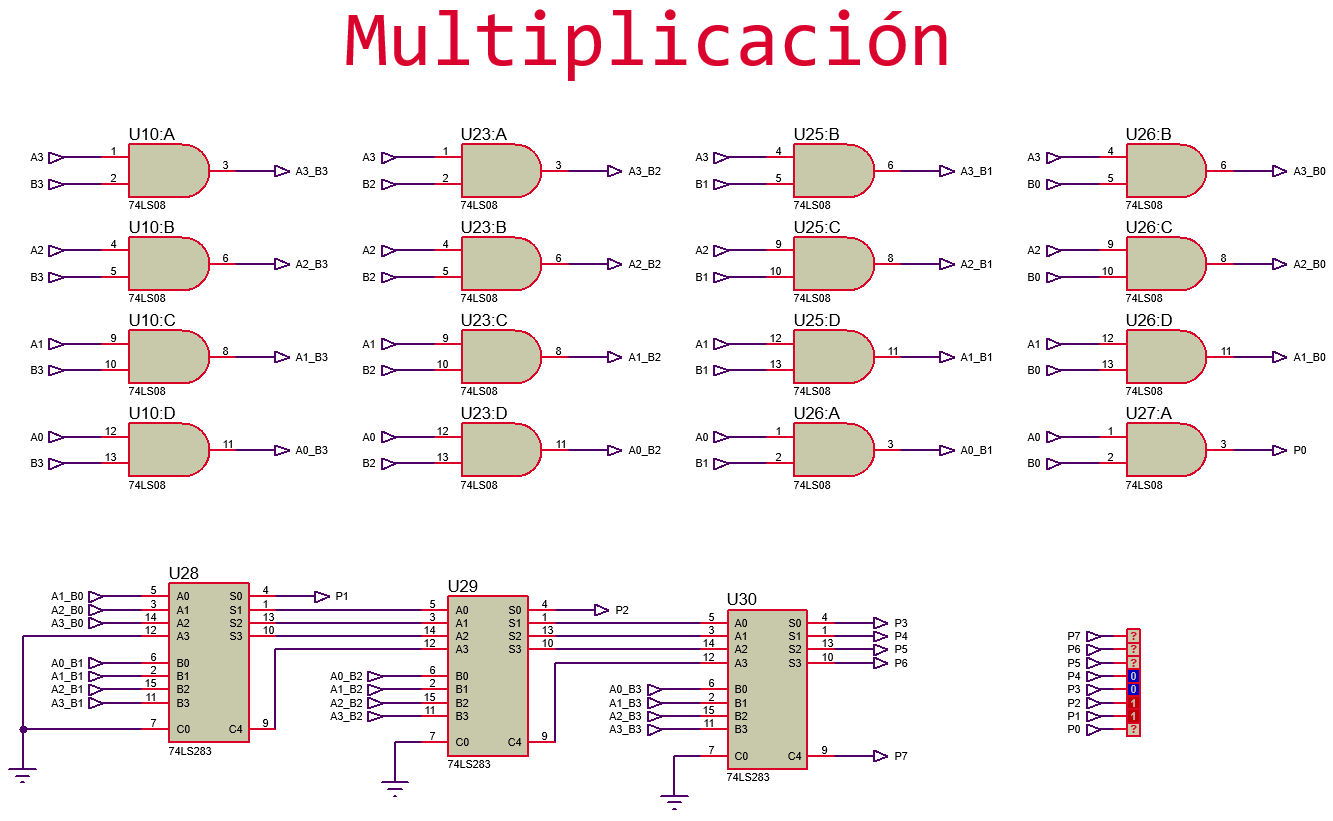
\includegraphics[width=\textwidth]{assets/multiplicacion.png}
    \caption{Módulo de multiplicación binaria.}
\end{figure}

\subsection{Módulo de potencia}
El bloque de potencia calcula $A^2$ y $A^3$. Para el cuadrado se generan productos parciales internos del mismo operando y se consolidan con sumadores. Para el cubo se reutilizan resultados del cuadrado y se extienden con una etapa adicional de combinación y suma.

\begin{table}[H]
    \centering
    \caption{Criterio de funcionamiento del bloque de potencia.}
    \begin{tabular}{c p{10cm}}
        \toprule
        \textbf{Valor de $B$} & \textbf{Operación realizada} \\
        \midrule
        0010 & El sistema calcula $A^2$, es decir, el cuadrado del operando $A$. \\
        0011 & El sistema calcula $A^3$, es decir, el cubo del operando $A$. \\
        Otro valor & No corresponde a los casos principales definidos para potencia dentro de esta práctica. \\
        \bottomrule
    \end{tabular}
\end{table}

\begin{table}[H]
    \centering
    \caption{Ejemplos de resultados de potencia en binario.}
    \small
    \begin{tabular}{>{\centering\arraybackslash}p{1.8cm} >{\centering\arraybackslash}p{1.6cm} >{\centering\arraybackslash}p{2.2cm} >{\centering\arraybackslash}p{2.6cm} p{3.8cm}}
        \toprule
        \textbf{$A$ bin} & \textbf{$B$} & \textbf{Operación} & \textbf{Resultado bin} & \textbf{Resultado decimal} \\
        \midrule
        0010 & 0010 & $2^2$ & 000100 & 4 \\
        0011 & 0010 & $3^2$ & 001001 & 9 \\
        0010 & 0011 & $2^3$ & 001000 & 8 \\
        0011 & 0011 & $3^3$ & 011011 & 27 \\
        \bottomrule
    \end{tabular}
\end{table}

\begin{table}[H]
    \centering
    \caption{Ficha del módulo de potencia.}
    \begin{tabular}{p{3.6cm}p{10cm}}
        \toprule
        \textbf{Elemento} & \textbf{Descripción} \\
        \midrule
        Integrados usados & 74LS08, 74LS283 y 74LS157 \\
        Entradas & $A[3:0]$, $B[3:0]$ y \texttt{op\_pow} \\
        Salidas & \texttt{POW0} a \texttt{POW5} \\
        Función & Selecciona y calcula el cuadrado o cubo del operando $A$ \\
        \bottomrule
    \end{tabular}
\end{table}

\begin{figure}[H]
    \centering
    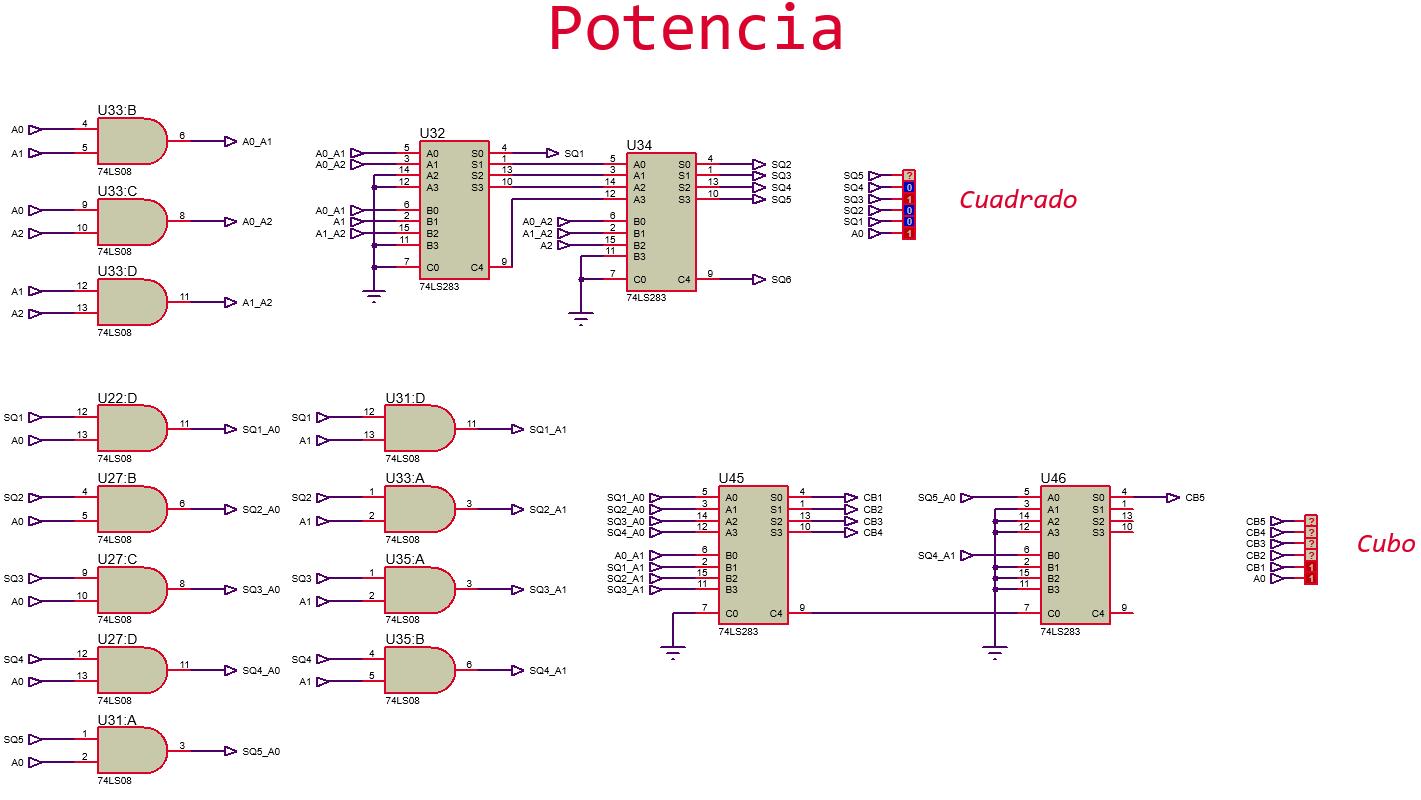
\includegraphics[width=\textwidth]{assets/potencia.png}
    \caption{Módulo de potencia para cuadrado y cubo.}
\end{figure}

\begin{figure}[H]
    \centering
    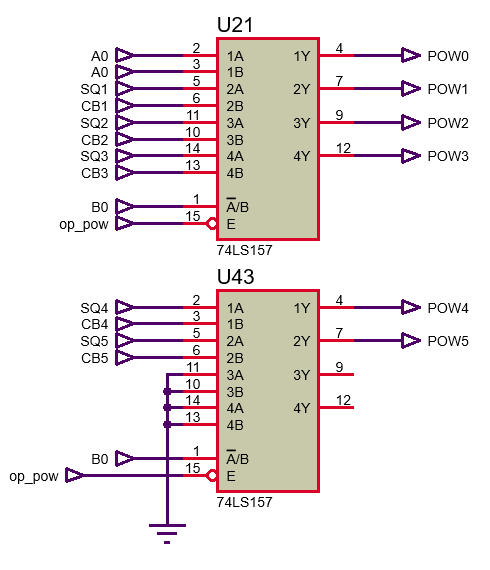
\includegraphics[width=0.48\textwidth]{assets/potencia_salidas.png}
    \caption{Selección de salidas del módulo de potencia.}
\end{figure}

\subsection{Unidad lógica}
La unidad lógica produce cuatro operaciones bit a bit: AND, OR, NAND y XNOR. Cada grupo procesa las cuatro líneas de entrada y luego consolida su salida hacia un LED de visualización por posición. La implementación es completamente combinacional y responde de manera inmediata a las entradas.

\begin{table}[H]
    \centering
    \caption{Tabla de verdad de las operaciones lógicas implementadas.}
    \begin{tabular}{c c c c c c}
        \toprule
        \textbf{A} & \textbf{B} & \textbf{AND} & \textbf{OR} & \textbf{NAND} & \textbf{XNOR} \\
        \midrule
        0 & 0 & 0 & 0 & 1 & 1 \\
        0 & 1 & 0 & 1 & 1 & 0 \\
        1 & 0 & 0 & 1 & 1 & 0 \\
        1 & 1 & 1 & 1 & 0 & 1 \\
        \bottomrule
    \end{tabular}
\end{table}

\begin{table}[H]
    \centering
    \caption{Resumen de visualización de la unidad lógica.}
    \begin{tabular}{p{4cm}p{9cm}}
        \toprule
        \textbf{Operación} & \textbf{Descripción de salida} \\
        \midrule
        AND & Enciende cada LED unicamente cuando el bit correspondiente de $A$ y $B$ vale 1. \\
        OR & Enciende el LED cuando al menos uno de los bits comparados es 1. \\
        NAND & Entrega la negación de AND, por lo que el LED se apaga solo cuando ambos bits son 1. \\
        XNOR & Enciende el LED cuando ambos bits son iguales. \\
        \bottomrule
    \end{tabular}
\end{table}

\begin{table}[H]
    \centering
    \caption{Ficha de la unidad lógica.}
    \begin{tabular}{p{3.6cm}p{10cm}}
        \toprule
        \textbf{Elemento} & \textbf{Descripción} \\
        \midrule
        Integrados usados & 74LS08, 74LS32, 74LS00 y 74LS266 \\
        Entradas & $A[3:0]$ y $B[3:0]$ \\
        Salidas & LEDs asociados a las cuatro operaciones lógicas \\
        Función & Evalúa operaciones lógicas bit a bit y las presenta visualmente \\
        \bottomrule
    \end{tabular}
\end{table}

\begin{figure}[H]
    \centering
    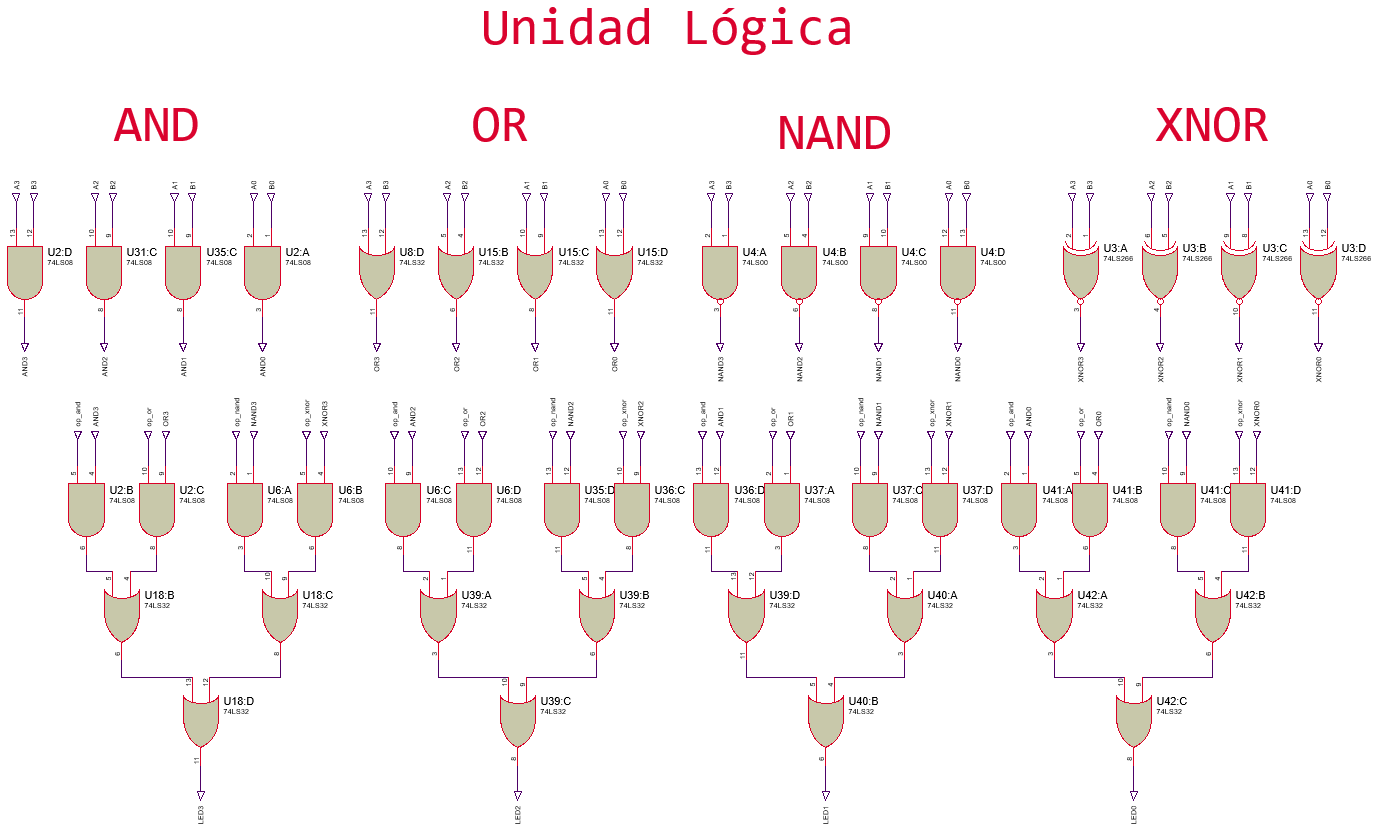
\includegraphics[width=\textwidth]{assets/unidad_logica.png}
    \caption{Unidad lógica del sistema.}
\end{figure}

\subsection{Unidad comparativa}
La unidad comparativa se construyó con un comparador 74LS85 y multiplexores 74LS157. El comparador determina si $A$ es mayor, igual o menor que $B$; con base en ello, los multiplexores enrutan el valor mayor a un display y el menor al otro. Si ambos operandos son iguales, ambos displays muestran el mismo número.

\begin{table}[H]
    \centering
    \caption{Tabla funcional de la unidad comparativa.}
    \begin{tabular}{p{3cm}p{5cm}p{5cm}}
        \toprule
        \textbf{Condición} & \textbf{Display superior} & \textbf{Display inferior} \\
        \midrule
        $A > B$ & Muestra $A$ como dígito mayor & Muestra $B$ como dígito menor \\
        $A < B$ & Muestra $B$ como dígito mayor & Muestra $A$ como dígito menor \\
        $A = B$ & Muestra $A$ & Muestra $A$ \\
        \bottomrule
    \end{tabular}
\end{table}

\begin{table}[H]
    \centering
    \caption{Ficha de la unidad comparativa.}
    \begin{tabular}{p{3.6cm}p{10cm}}
        \toprule
        \textbf{Elemento} & \textbf{Descripción} \\
        \midrule
        Integrados usados & 74LS85, 74LS157 y 74LS48 \\
        Entradas & $A[3:0]$ y $B[3:0]$ \\
        Salidas & Dos displays de siete segmentos: mayor y menor \\
        Función & Determina la relación entre operandos y presenta el mayor y el menor \\
        \bottomrule
    \end{tabular}
\end{table}

\begin{figure}[H]
    \centering
    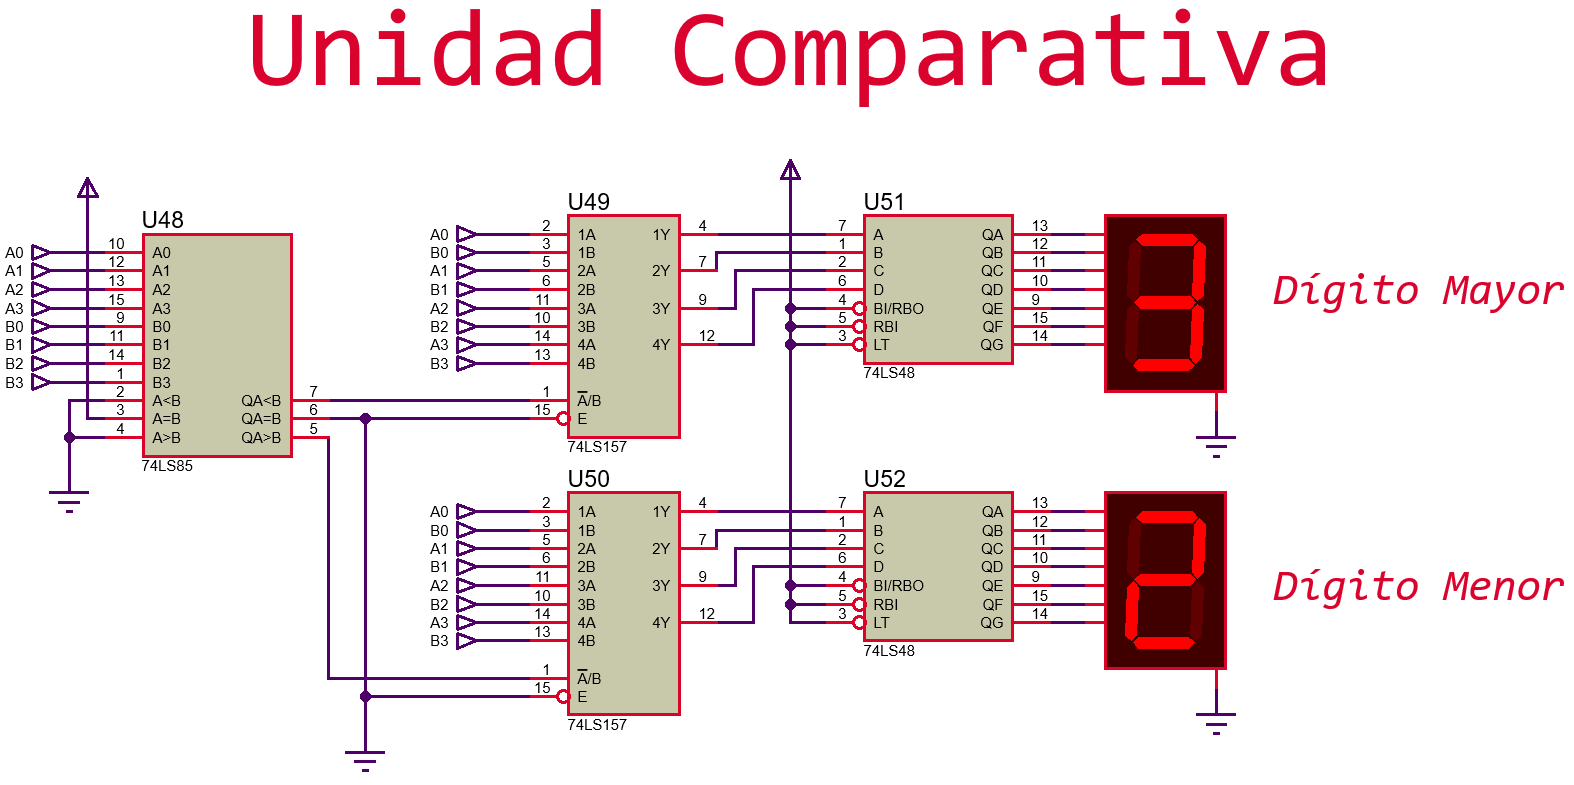
\includegraphics[width=\textwidth]{assets/unidad_comparativa.png}
    \caption{Unidad comparativa para mostrar dígito mayor y menor.}
\end{figure}

\subsection{Conversión de binario a BCD y visualización}
Para mostrar resultados aritméticos en displays de siete segmentos se incorporó un bloque de conversión de binario a BCD. Este bloque recibe resultados de suma, resta y multiplicación, realiza combinaciones intermedias y adapta la información a decodificadores 74LS48 para alimentar los displays.

\begin{table}[H]
    \centering
    \caption{Rutas principales consideradas en la etapa binario a BCD.}
    \begin{tabular}{p{4cm}p{9cm}}
        \toprule
        \textbf{Ruta de entrada} & \textbf{Uso dentro del conversor} \\
        \midrule
        \texttt{RES[3:0]} & Resultado de suma o resta en 4 bits. \\
        \texttt{RES\_COUT} & Bit adicional de acarreo para resultados aritméticos. \\
        \texttt{P[7:0]} & Resultado expandido de la multiplicación. \\
        \texttt{POW[5:0]} & Resultado proveniente del bloque de potencia. \\
        \texttt{sign\_bit} & Indicador asociado a la resta para ajuste de presentacion. \\
        \bottomrule
    \end{tabular}
\end{table}

\begin{table}[H]
    \centering
    \caption{Ficha del bloque binario a BCD.}
    \begin{tabular}{p{3.6cm}p{10cm}}
        \toprule
        \textbf{Elemento} & \textbf{Descripción} \\
        \midrule
        Integrados usados & 74LS86, 74LS08, 74LS32, 74LS283 y 74LS48 \\
        Entradas & Resultados de suma, resta, multiplicación y señales de selección \\
        Salidas & Bits BCD y señales hacia displays de siete segmentos \\
        Función & Traduce resultados binarios a una forma visual legible en decimal \\
        \bottomrule
    \end{tabular}
\end{table}

\begin{figure}[H]
    \centering
    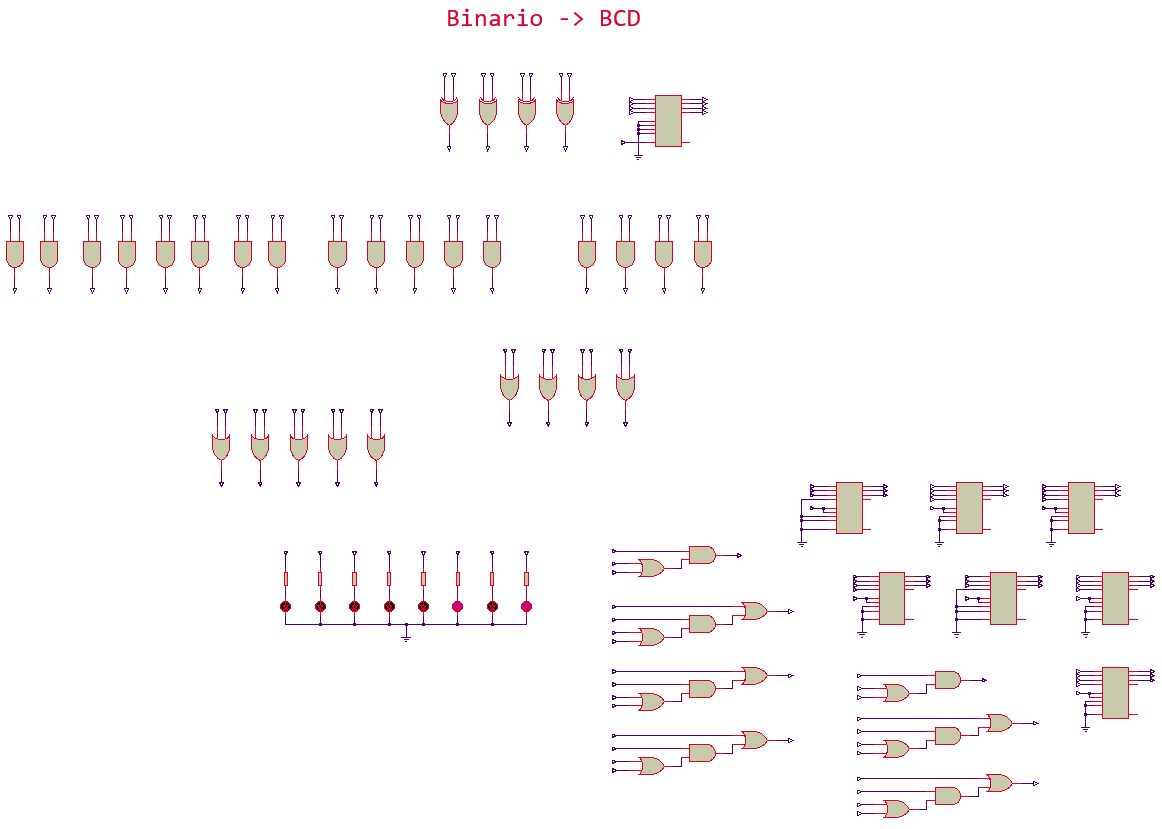
\includegraphics[width=\textwidth]{assets/binario_bcd_vista_general.png}
    \caption{Vista general del bloque binario a BCD.}
\end{figure}

\begin{figure}[H]
    \centering
    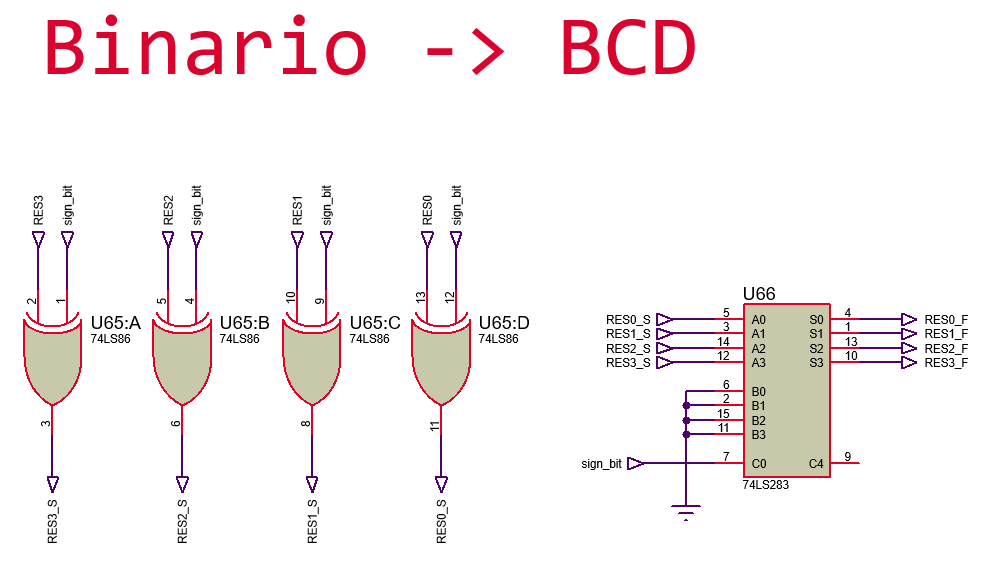
\includegraphics[width=\textwidth]{assets/binario_bcd_p1.png}
    \caption{Primera etapa de conversión binario a BCD.}
\end{figure}

\begin{figure}[H]
    \centering
    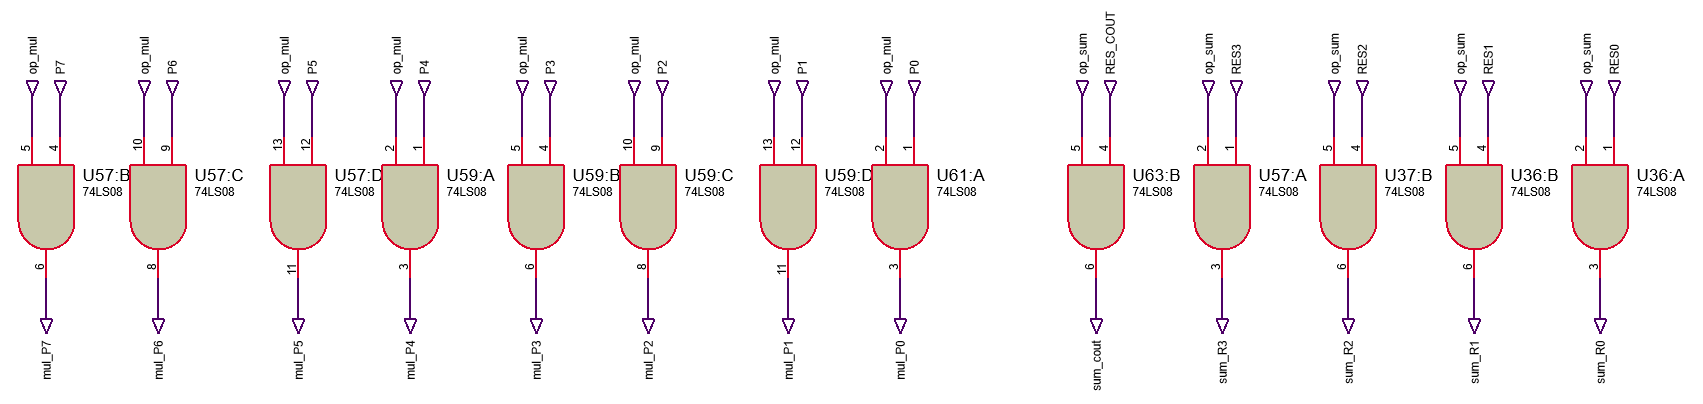
\includegraphics[width=\textwidth]{assets/binario_bcd_p2.png}
    \caption{Filtrado y enrutamiento de líneas por operación activa.}
\end{figure}

\begin{figure}[H]
    \centering
    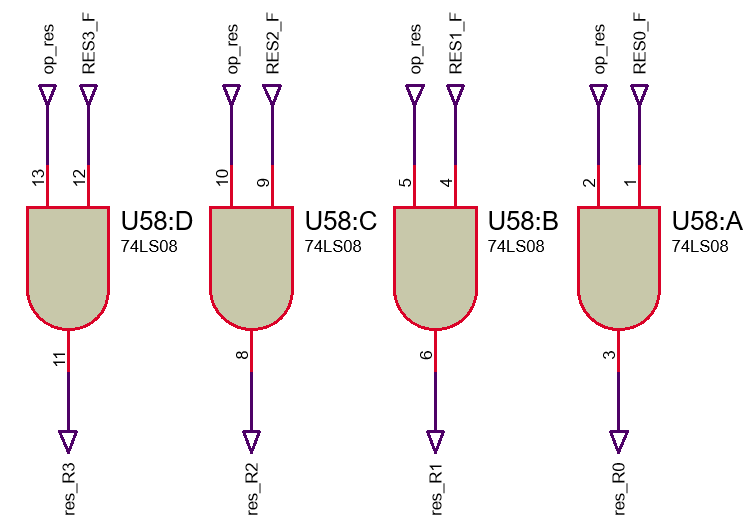
\includegraphics[width=0.8\textwidth]{assets/binario_bcd_p3.png}
    \caption{Acondicionamiento de líneas para la resta.}
\end{figure}

\begin{figure}[H]
    \centering
    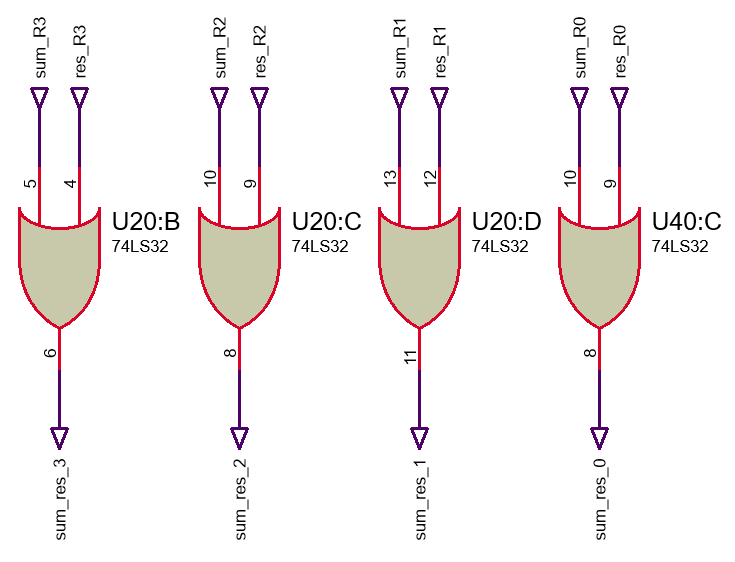
\includegraphics[width=0.78\textwidth]{assets/binario_bcd_p4.png}
    \caption{Combinación entre resultados de suma y resta.}
\end{figure}

\begin{figure}[H]
    \centering
    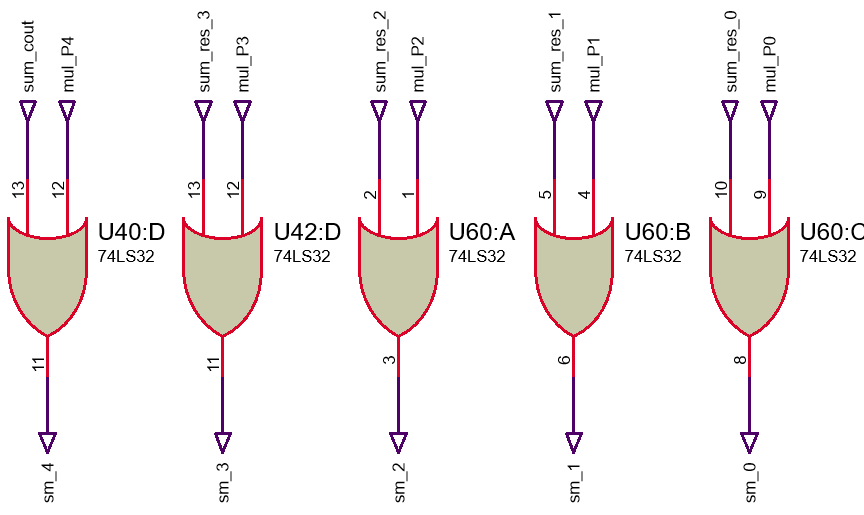
\includegraphics[width=0.92\textwidth]{assets/binario_bcd_p5.png}
    \caption{Combinación entre resultados de multiplicación y suma/resta.}
\end{figure}

\begin{figure}[H]
    \centering
    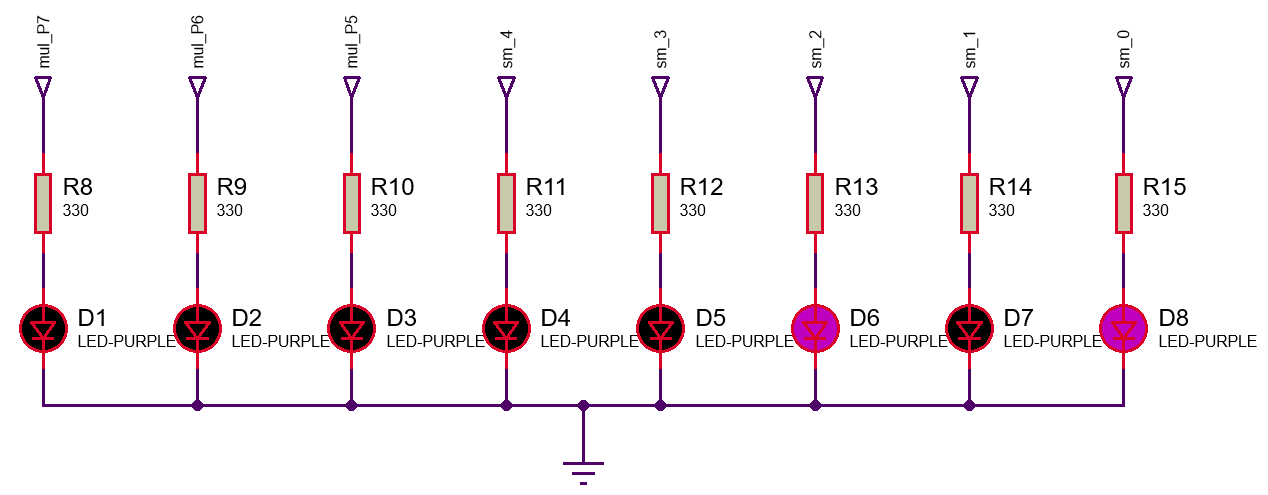
\includegraphics[width=\textwidth]{assets/binario_bcd_p6.png}
    \caption{Banco de LEDs de prueba para salidas intermedias.}
\end{figure}

\begin{figure}[H]
    \centering
    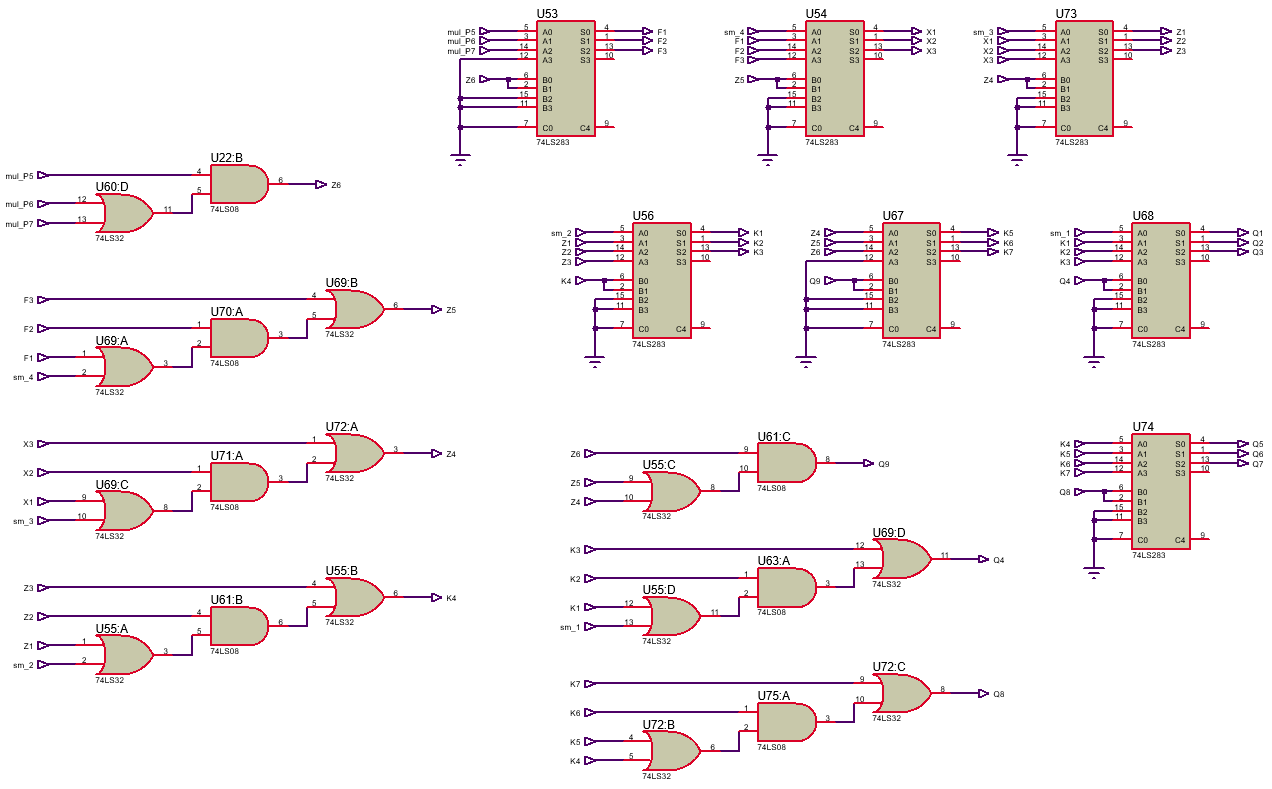
\includegraphics[width=\textwidth]{assets/binario_bcd_p7.png}
    \caption{Etapas finales del conversor y propagacion a buses de salida.}
\end{figure}

\subsection{Visualización de resultados}
La validación final incluyó displays para los resultados aritméticos y LEDs para estados binarios. En la captura siguiente se observa una configuración de prueba donde la salida aritmética y el grupo de potencia son visibles de manera simultánea.

\begin{figure}[H]
    \centering
    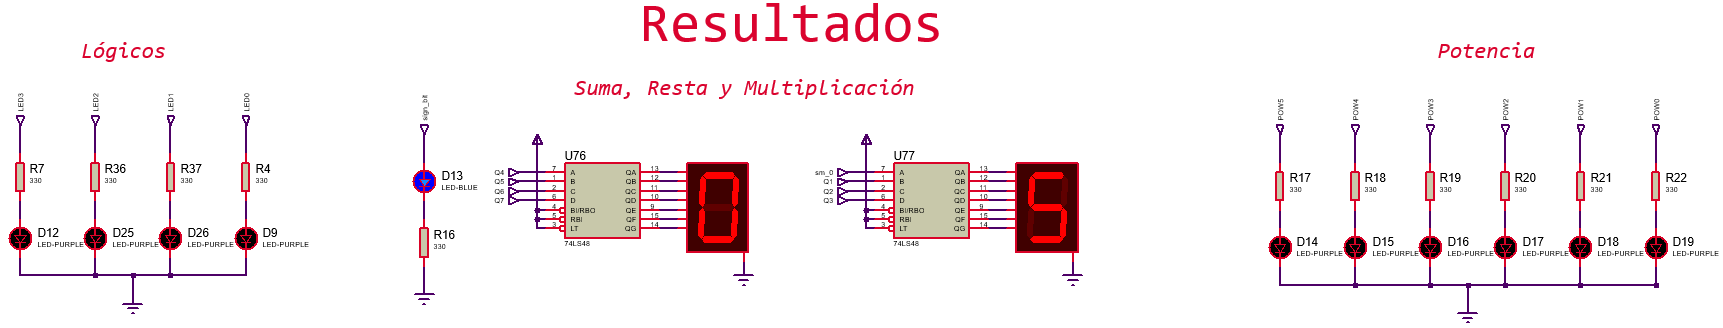
\includegraphics[width=\textwidth]{assets/resultados.png}
    \caption{Captura general de resultados en el esquema.}
\end{figure}

\section{Implementación Física}
Además del diseño en Proteus, se realizó el montaje en protoboards. El ensamble físico evidencia la complejidad del sistema debido a la cantidad de interconexiones, compuertas y bloques funcionales involucrados. Se utilizaron varios protoboards, cableado de colores y encapsulados TTL discretos para sostener la implementación modular.

\begin{figure}[H]
    \centering
    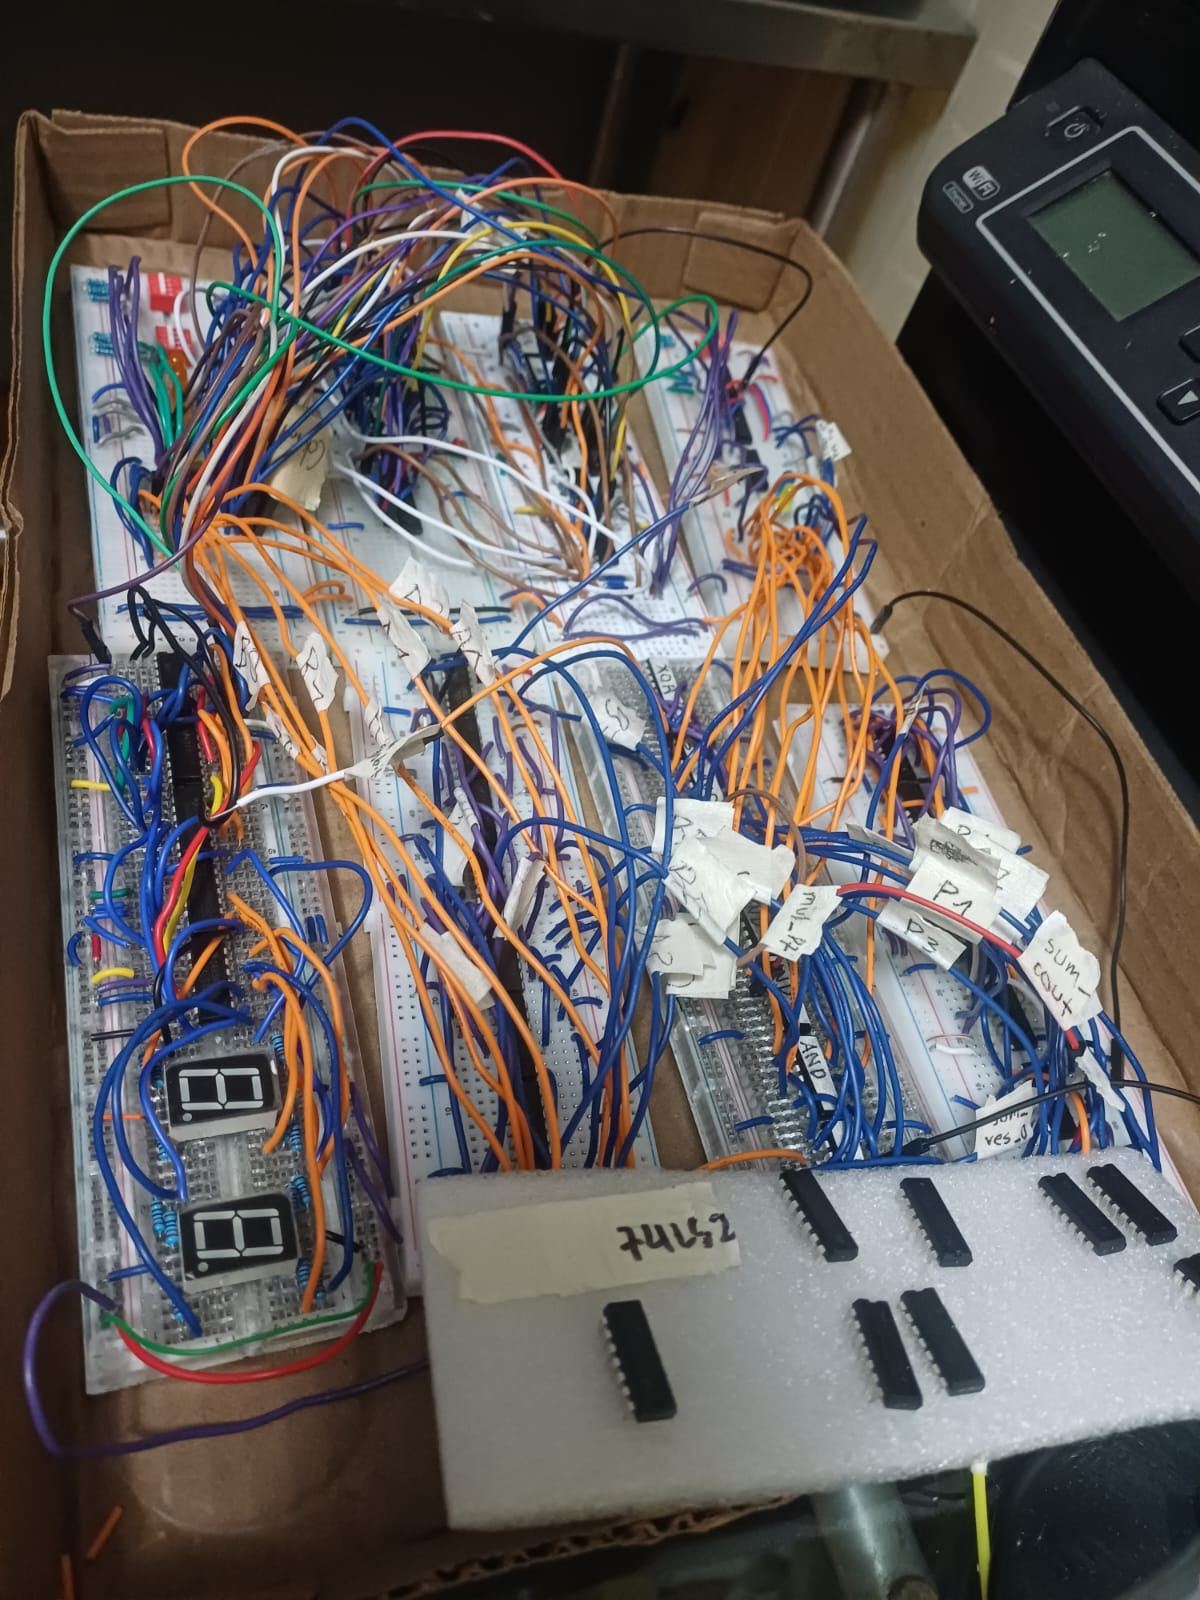
\includegraphics[width=0.7\textwidth]{assets/frame.jpeg}
    \caption{Montaje físico principal en protoboards.}
\end{figure}

\section{Material de apoyo}
Los recursos mencionados en el enunciado y utilizados como referencia conceptual durante la práctica incluyen:
\begin{itemize}[leftmargin=1.2cm]
    \item Proteus Design Suite: \url{https://www.labcenter.com/downloads/}
    \item Mapas de Karnaugh y simplificación booleana: \url{https://www.ingmecafenix.com/electronica/digital/mapa-de-karnaugh/}
    \item Material audiovisual de apoyo compartido en el enunciado: \url{https://youtu.be/nNMngrtd_XA?si=Vtezv8atgSqr_Ta9}
\end{itemize}

\section{Recursos y herramientas utilizadas}
\begin{itemize}[leftmargin=1.2cm]
    \item Simulador Proteus, utilizado para el desarrollo, integración y depuración del circuito.
    \item Integrados TTL de la serie 74LS, empleados en los módulos aritméticos, lógicos, comparativos y de visualización.
    \item Displays de siete segmentos de cátodo común, usados para mostrar resultados numéricos.
    \item LEDs de distintos colores, utilizados como indicadores de estado y salidas lógicas.
    \item Resistencias de polarización y limitación de corriente, necesarias para estabilizar entradas y proteger indicadores.
    \item Protoboards y cables jumper, usados en la implementación física del sistema.
    \item Factura de compra, utilizada como respaldo para la sección de presupuesto.
\end{itemize}

\section{Cronograma de trabajo}
El desarrollo de la práctica se puede resumir en el siguiente cronograma ejecutado:

\begin{longtable}{p{3.5cm}p{11cm}}
\toprule
\textbf{Fecha} & \textbf{Actividad principal} \\
\midrule
17 de marzo de 2026 & Compra de componentes y obtención del material electrónico base, según la factura proporcionada. \\
18 al 19 de marzo de 2026 & Diseño de bloques funcionales en Proteus: controlador, entradas, suma/resta, lógica y comparación. \\
20 al 21 de marzo de 2026 & Integración de multiplicación, potencia, conversión binario a BCD y validación visual de salidas. \\
21 al 22 de marzo de 2026 & Montaje físico en protoboards, captura de evidencias y elaboración de la documentación. \\
\bottomrule
\end{longtable}

\section{Presupuesto}
La siguiente tabla fue elaborada a partir de la factura fotografiada de Electrónica Sigma Guatemala.

\begin{longtable}{p{6.2cm}c c c}
\toprule
\textbf{Producto} & \textbf{Cantidad} & \textbf{Precio} & \textbf{Total} \\
\midrule
DIP switch de 4 posiciones & 2 & Q3.75 & Q7.50 \\
Decodificador / demultiplexor 74LS138 & 1 & Q6.00 & Q6.00 \\
LED azul difuso 5 mm & 1 & Q1.00 & Q1.00 \\
LED amarillo difuso 5 mm & 1 & Q1.00 & Q1.00 \\
LED naranja difuso 5 mm & 11 & Q1.00 & Q11.00 \\
Compuerta lógica NAND 74LS00 & 2 & Q5.00 & Q10.00 \\
Comparador 74LS85 & 1 & Q11.00 & Q11.00 \\
Multiplexor 74LS157 & 4 & Q7.00 & Q28.00 \\
Decodificador / driver para 7 segmentos 74LS48, cátodo común & 4 & Q9.00 & Q36.00 \\
Display de 7 segmentos, cátodo común rojo & 2 & Q5.00 & Q10.00 \\
Compuerta lógica XOR 74LS86 & 5 & Q6.00 & Q30.00 \\
Sumador de 4 bits 74LS283 & 15 & Q14.00 & Q210.00 \\
Compuerta lógica AND 74LS08 & 4 & Q5.00 & Q20.00 \\
Compuerta lógica XNOR 74LS266 & 2 & Q12.00 & Q24.00 \\
\midrule
\textbf{Subtotal} & & & \textbf{Q405.50} \\
\textbf{Total} & & & \textbf{Q405.50} \\
\textbf{Efectivo entregado} & & & \textbf{Q410.50} \\
\textbf{Cambio} & & & \textbf{Q5.00} \\
\bottomrule
\end{longtable}

\section{Resultados y observaciones}
El prototipo cumple con la estructura solicitada para una ALU básica discreta. La separación por módulos facilita el análisis del funcionamiento y permite probar cada operación por separado. Entre los resultados más relevantes destacan los siguientes:
\begin{itemize}[leftmargin=1.2cm]
    \item La selección de operaciones se controla desde un bloque central único.
    \item Las entradas binarias son estables y fáciles de modificar mediante DIP switches.
    \item La unidad lógica ofrece una visualización inmediata por LEDs.
    \item La unidad comparativa resuelve correctamente la selección entre mayor y menor.
    \item La unidad aritmética logra operaciones simples y compuestas, aunque a costa de un alto número de integrados y cableado.
\end{itemize}

Como observación técnica, la parte más demandante del proyecto fue la integración entre la lógica aritmética y la visualización decimal. El bloque binario a BCD y la multiplexación de resultados aumentan significativamente la complejidad del diseño.

\section{Conclusiones}
\begin{itemize}[leftmargin=1.2cm]
    \item Se implementó una calculadora digital modular de 4 bits basada exclusivamente en lógica combinacional y circuitos TTL.
    \item La práctica permitió comprobar que una ALU básica puede construirse por bloques funcionales claramente diferenciados: control, aritmética, lógica, comparación y visualización.
    \item La simulación en Proteus fue esencial para depurar conexiones antes de trasladar el circuito a protoboards.
    \item El montaje físico evidencia el costo real en espacio, componentes y complejidad cuando se resuelve un problema digital sin elementos programables.
    \item La documentación y el presupuesto complementan la solución técnica al dejar trazabilidad del proceso de construcción.
\end{itemize}

\section{Anexos}

\subsection{Capturas del montaje físico}

\begin{figure}[H]
    \centering
    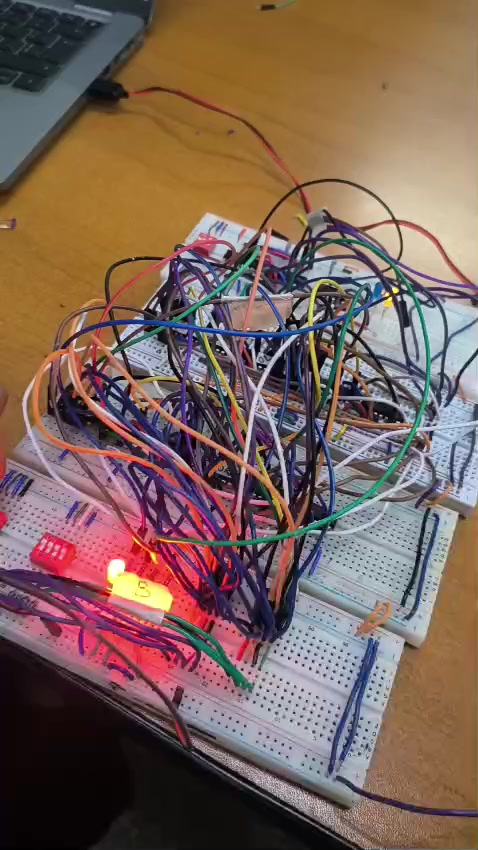
\includegraphics[width=0.74\textwidth]{assets/frame_000001.jpg}
    \caption{Anexo A. Vista del montaje físico.}
\end{figure}

\begin{figure}[H]
    \centering
    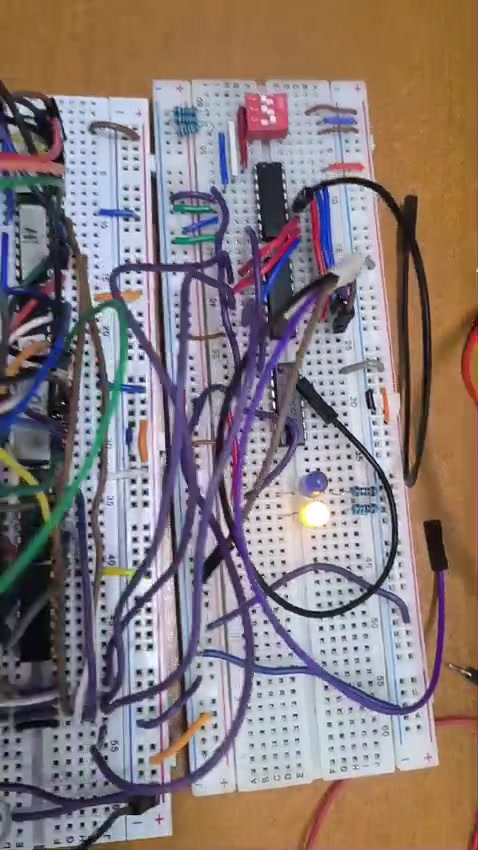
\includegraphics[width=0.74\textwidth]{assets/frame_000048.jpg}
    \caption{Anexo B. Detalle del montaje físico.}
\end{figure}

\begin{figure}[H]
    \centering
    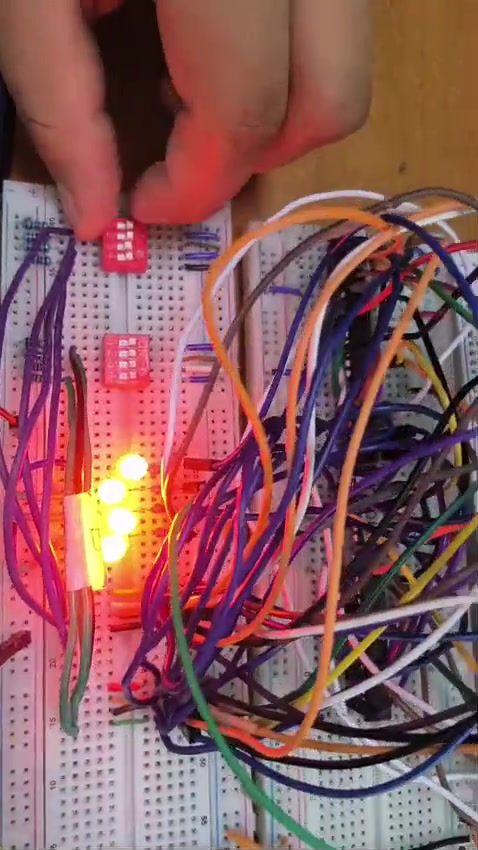
\includegraphics[width=0.74\textwidth]{assets/frame_000118.jpg}
    \caption{Anexo C. Evidencia adicional del prototipo.}
\end{figure}

\begin{figure}[H]
    \centering
    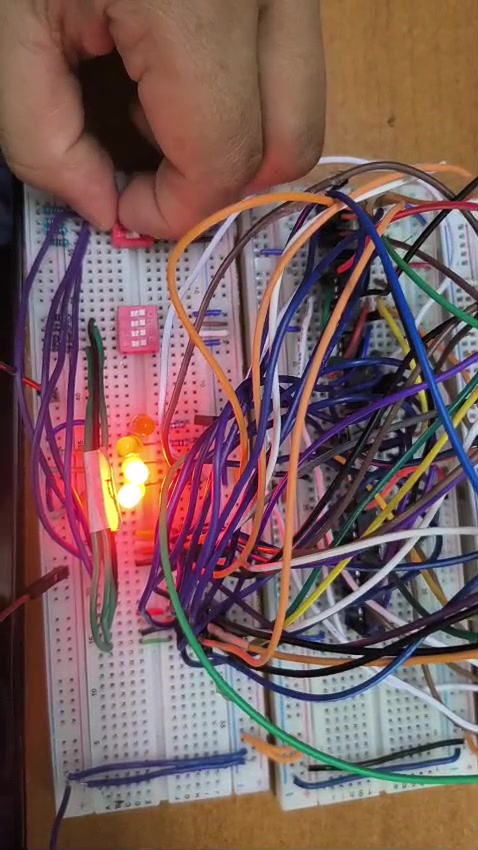
\includegraphics[width=0.74\textwidth]{assets/frame_000241.jpg}
    \caption{Anexo D. Conexionado del sistema.}
\end{figure}

\begin{figure}[H]
    \centering
    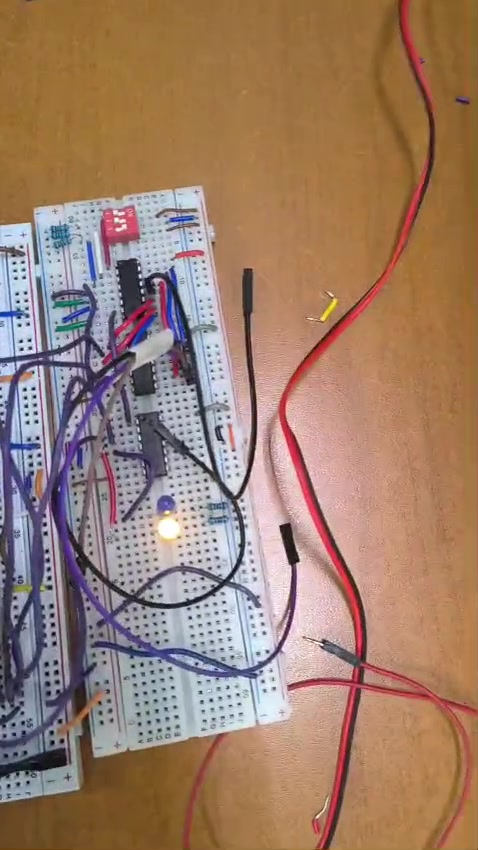
\includegraphics[width=0.74\textwidth]{assets/frame_000384.jpg}
    \caption{Anexo E. Integración de módulos en protoboard.}
\end{figure}

\begin{figure}[H]
    \centering
    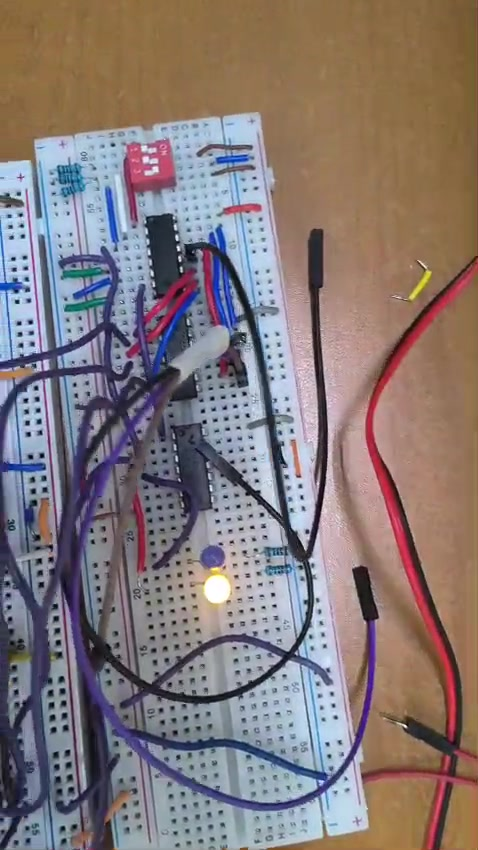
\includegraphics[width=0.74\textwidth]{assets/frame_000410.jpg}
    \caption{Anexo F. Vista final del montaje.}
\end{figure}

\subsection{Factura}
\begin{figure}[H]
    \centering
    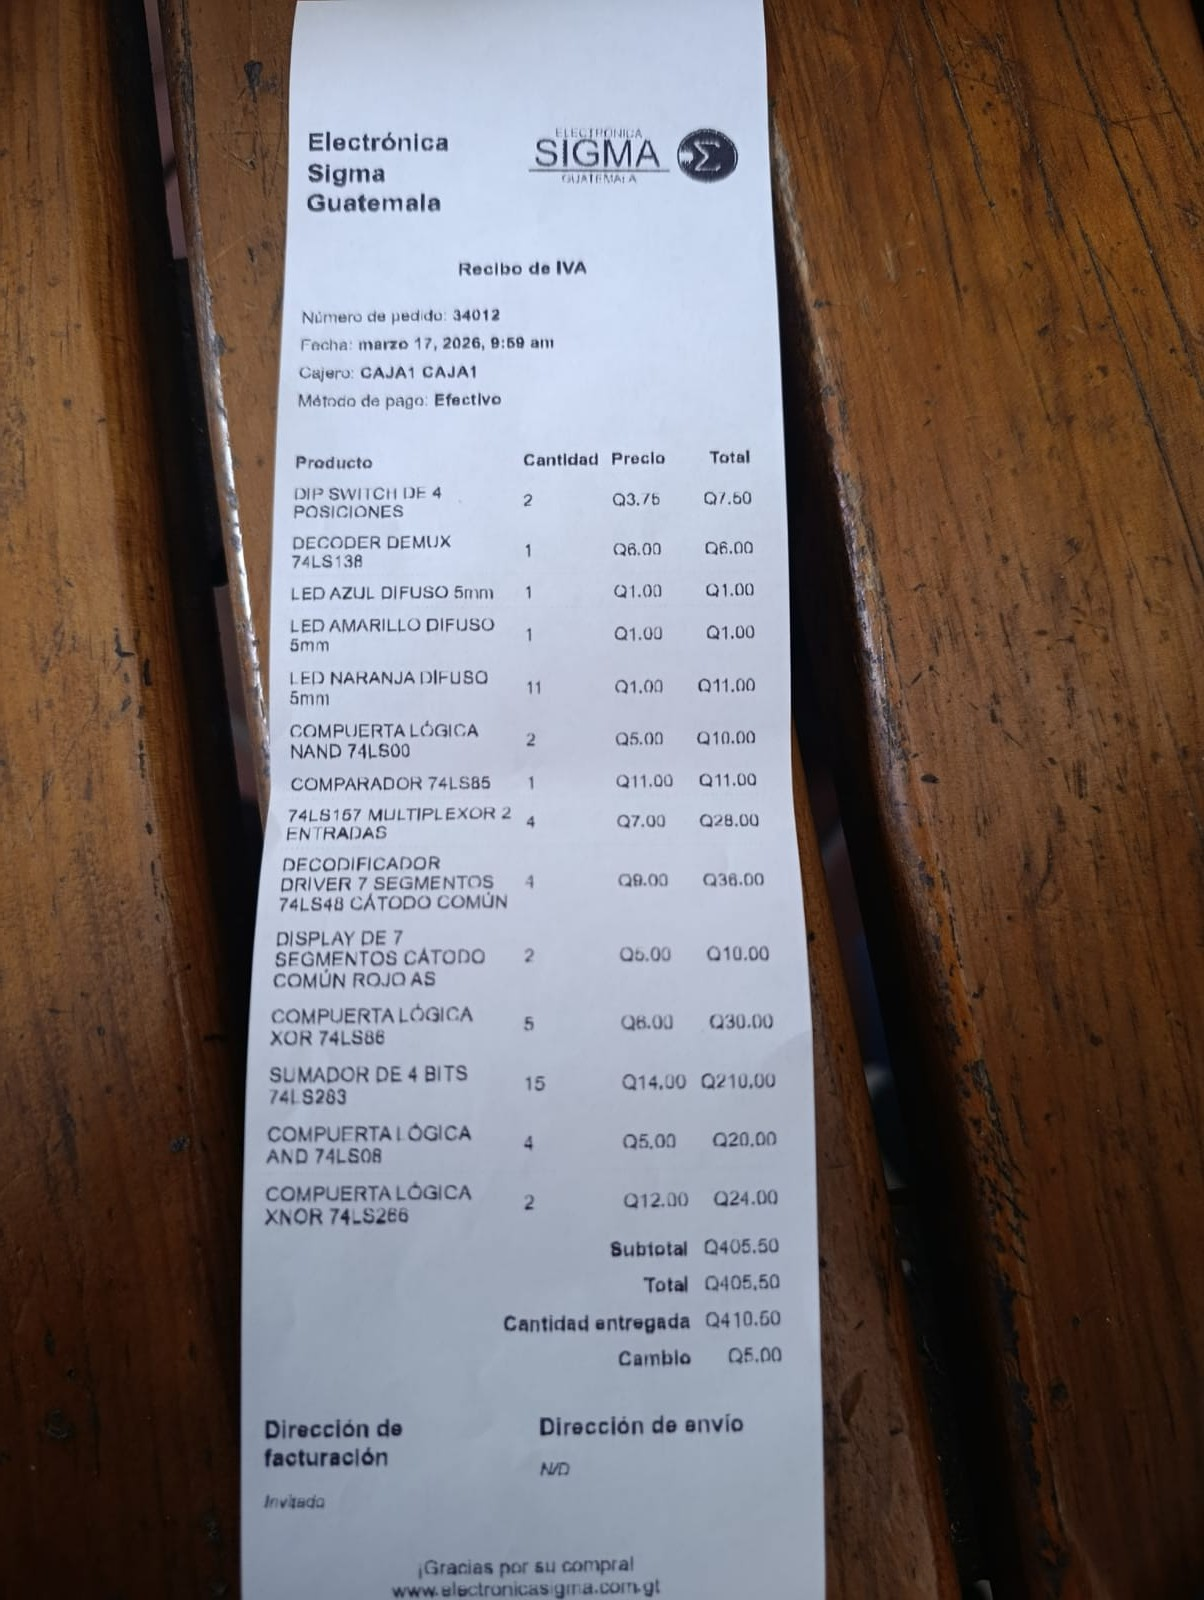
\includegraphics[width=0.48\textwidth]{assets/factura.jpeg}
    \caption{Anexo G. Factura utilizada para la elaboración del presupuesto.}
\end{figure}

\end{document}
